
\documentclass[8pt]{beamer}
\usetheme{default}
\PassOptionsToPackage{usenames,dvipsnames}{xcolor}
\usepackage{my_pres}
\usepackage{tikz}
\usepackage{empheq,accents}
\usepackage{pifont}
\usetikzlibrary{arrows}



% Created by S. Boyd and L. Vandenberghe 
% some traditional definitions that can be blamed on craig barratt
\newcommand{\BEAS}{\begin{eqnarray*}}
\newcommand{\EEAS}{\end{eqnarray*}}
\newcommand{\BEA}{\begin{eqnarray}}
\newcommand{\EEA}{\end{eqnarray}}
\newcommand{\BEQ}{\begin{equation}}
\newcommand{\EEQ}{\end{equation}}
\newcommand{\BIT}{\begin{itemize}}
\newcommand{\EIT}{\end{itemize}}

% text abbrevs
\newcommand{\eg}{{\it e.g.}}
\newcommand{\ie}{{\it i.e.}}

% std math stuff
\newcommand{\ones}{\mathbf 1}
\newcommand{\reals}{{\mbox{\bf R}}}
\newcommand{\integers}{{\mbox{\bf Z}}}
\newcommand{\complex}{{\mbox{\bf C}}}
\newcommand{\symm}{{\mbox{\bf S}}}  % symmetric matrices

% lin alg stuff
\newcommand{\Span}{\mbox{\textrm{span}}}
\newcommand{\range}{{\mathcal R}}
\newcommand{\nullspace}{{\mathcal N}}
\newcommand{\Rank}{\mathop{\bf rank}}
\newcommand{\Tr}{\mathop{\bf tr}}
\newcommand{\cond}{\mathop{\bf cond}}
\newcommand{\diag}{\mathop{\bf diag}}
\newcommand{\lambdamax}{\lambda_{\rm max}}
\newcommand{\lambdamin}{\lambda_{\rm min}}

% probability stuff
\newcommand{\Prob}{\mathop{\bf prob}}
\newcommand{\Expect}{\mathop{\bf E{}}}
\newcommand{\var}{\mathop{\bf var}} % variance
% not sure why we have \Expect and \Prob but \var ???

% convexity & optimization stuff
\newcommand{\Co}{\mathop {\bf conv}} % convex hull
\newcommand{\argmin}{\mathop{\rm argmin}}
\newcommand{\argmax}{\mathop{\rm argmax}}
\newcommand{\epi}{\mathop{\bf epi}}
%\newcommand{\hypo}{\mathop{\bf hypo}}

% sup and inf that look OK in saddle-point form!
%\newcommand{\ourinf}{\mathop{\raisebox{0ex}[0ex][.4ex]{\,inf\,}}}
%\newcommand{\oursup}{\mathop{\raisebox{0ex}[0ex][.4ex]{\,sup\,}}}
\newcommand{\ourinf}{\mathop{\,\mathrm{inf}\, {\rule[-.5ex]{0ex}{0ex}}}}
\newcommand{\oursup}{\mathop{\,\mathrm{sup}\, {\rule[-.5ex]{0ex}{0ex}}}}
%makes latex believe that inf and sup both extend .4ex below
%the baseline

\newcommand{\dist}{\mathop{\bf dist}}
\newcommand{\vol}{\mathop{\bf vol}} % volume
\newcommand{\Card}{\mathop{\bf card}} % cardinality
\newcommand{\sign}{\mathop{\bf sign}}

\newcommand{\dom}{\mathop{\bf dom}} % domain
\newcommand{\aff}{\mathop{\bf aff}} % affine hull
\newcommand{\cl}{\mathop{\bf cl}} % closure
\newcommand{\intr}{\mathop{\bf int}} % interior
\newcommand{\relint}{\mathop{\bf rel int}} % relative interior
\newcommand{\bd}{\mathop{\bf bd}} % boundary

%why do we have the following but not \nust?
\newcommand{\xst}{x^\star}
\newcommand{\lambdast}{\lambda^\star}

% defs for cones & generalized inequalities
% these seem kind of awkward; should fix some day
% rewrite them to use args?
\newcommand{\geqK}{\mathrel{\succeq_K}}
\newcommand{\gK}{\mathrel{\succ_K}}
\newcommand{\leqK}{\mathrel{\preceq_K}}
\newcommand{\lK}{\mathrel{\prec_K}}
\newcommand{\geqKst}{\mathrel{\succeq_{K^*}}}
\newcommand{\gKst}{\mathrel{\succ_{K^*}}}
\newcommand{\leqKst}{\mathrel{\preceq_{K^*}}}
\newcommand{\lKst}{\mathrel{\prec_{K^*}}}
\newcommand{\geqL}{\mathrel{\succeq_L}}
\newcommand{\gL}{\mathrel{\succ_L}}
\newcommand{\leqL}{\mathrel{\preceq_L}}
\newcommand{\lL}{\mathrel{\prec_L}}
\newcommand{\geqLst}{\mathrel{\succeq_{L^*}}}
\newcommand{\gLst}{\mathrel{\succ_{L^*}}}
\newcommand{\leqLst}{\mathrel{\preceq_{L^*}}}
\newcommand{\lLst}{\mathrel{\prec_{L^*}}}

%\newcounter{lecture}
%\newcommand{\lecturefl}[1]{   % use with foiltex landscape
%% \addtocounter{lecture}{1}
% \refstepcounter{lecture}
% \setcounter{equation}{0}
% \setcounter{page}{1}
% \renewcommand{\theequation}{\arabic{equation}}
% \renewcommand{\thepage}{\arabic{lecture}--\arabic{page}}
% \raggedright
% \parindent 0pt
% \rightfooter{\thepage}
% \leftheader{}
% \rightheader{}
% \LogoOff
% \input header 
% \begin{center}
%% {\Large \bfseries Lecture \arabic{lecture} \\*[\bigskipamount] {#1}}
%{\Large \bfseries \arabic{lecture}.  {#1}}
% \end{center}
% \MyLogo{#1}
%}

%\newcommand{\lectureflstar}[1]{   % use with foiltex landscape
% \setcounter{equation}{0}
% \setcounter{page}{1}
% \renewcommand{\theequation}{\arabic{equation}}
% \renewcommand{\thepage}{\arabic{page}}
% \raggedright
% \parindent 0pt
% \rightfooter{\thepage}
% \leftheader{}
% \rightheader{}
% \LogoOff
% \input header 
% \begin{center}
% {\Large \bfseries #1}
% \end{center}
% \MyLogo{#1}
%}
%\newcounter{oursection}
%\newcommand{\frametitle}[1]{  % for use with foiltex landscape
% \addtocounter{oursection}{1}
%% \setcounter{equation}{0}
% \foilhead[-1.0cm]{#1}
% \LogoOn
%}

\newenvironment{algdesc}%
   {\begin{list}{}{%
    \setlength{\rightmargin}{0\linewidth}%
    \setlength{\leftmargin}{.05\linewidth}}%
    \sffamily\small
    \item[]{\setlength{\parskip}{0ex}\hrulefill\par%
    \nopagebreak{}}}%
   {{\setlength{\parskip}{-1ex}\nopagebreak\par\hrulefill} \end{list}}

\newenvironment{colm}{\left[\begin{array}{c}}{\end{array}\right]}
\newenvironment{colv}{\left(\begin{array}{c}}{\end{array}\right)}




\definecolor{texthigh}{RGB}{137, 0, 255}
\definecolor{textred}{RGB}{255, 0, 94}
\definecolor{textgreen}{RGB}{89, 232, 151}
\definecolor{textlightgray}{RGB}{170,170,170}
\definecolor{bggray}{RGB}{230,230,230}
\definecolor{textgray}{RGB}{60,60,60}

\setbeamercolor{background canvas}{bg=bggray}
\setbeamercolor{normal text}{fg=textgray}

\setbeamertemplate{enumerate items}[default]
\setbeamertemplate{itemize items}{\ding{84}}

\title{Informative Data Fusion:\\ Beyond Canonical Correlation Analysis}
\institute[Univ. of Michigan]{\texttt{asendorf@umich.edu}\\[3ex]
Department of Electrical Engineering and Computer
  Science\\University of Michigan\\ }
\author[N. Asendorf]{Nicholas Asendorf}
\date{Dissertation Defense\\[2ex] May 4, 2015}

\newcommand{\twr}{{\sf TW}_\reals}
\newcommand{\twc}{{\sf TW}_\complex}
\newcommand{\sx}{s_{x,i}}
\newcommand{\sy}{s_{y,i}}
\newcommand{\zx}{z_{x,i}}
\newcommand{\zy}{z_{y,i}}
\newcommand{\Zx}{Z_x}
\newcommand{\Zy}{Z_y}
\newcommand{\Ux}{U_x}
\newcommand{\Uy}{U_y}
\newcommand{\Vx}{V_x}
\newcommand{\Vy}{V_y}
\newcommand{\Pxy}{P_{xy}}
\newcommand{\kx}{k_x}
\newcommand{\ky}{k_y}
\newcommand{\kxhat}{\widehat{k}_x}
\newcommand{\kyhat}{\widehat{k}_y}
\newcommand{\khatcca}{\widehat{k}_{\text{cca}}}
\newcommand{\khaticca}{\widehat{k}_{\text{icca}}}
\newcommand{\Uxhat}{\widehat{U}_x}
\newcommand{\Uyhat}{\widehat{U}_y}
\newcommand{\Sigxhat}{\widehat{\Sigma}_x}
\newcommand{\Sigyhat}{\widehat{\Sigma}_y}
\newcommand{\Vxhat}{\widehat{V}_x}
\newcommand{\Vyhat}{\widehat{V}_y}
\newcommand{\Uxtil}{\widetilde{U}_x}
\newcommand{\Uytil}{\widetilde{U}_y}
\newcommand{\Vxtil}{\widetilde{V}_x}
\newcommand{\Vytil}{\widetilde{V}_y}
\newcommand{\Uxcir}{\accentset{\circ}{U}_x}
\newcommand{\Ukcir}{\accentset{\circ}{U}_{\widetilde{K}}}
\newcommand{\Uycir}{\accentset{\circ}{U}_y}
\newcommand{\Sigxcir}{\accentset{\circ}{\Sigma}_x}
\newcommand{\Sigycir}{\accentset{\circ}{\Sigma}_y}
\newcommand{\Vxcir}{\accentset{\circ}{V}_x}
\newcommand{\Vycir}{\accentset{\circ}{V}_y}
\newcommand{\kapcir}{\accentset{\circ}{\kappa}}
\newcommand{\xii}{x_i}
\newcommand{\yii}{y_i}
\newcommand{\Tx}{\Theta_x}
\newcommand{\Ty}{\Theta_y}
\newcommand{\Txhat}{\widehat{\Theta}_x}
\newcommand{\Tyhat}{\widehat{\Theta}_y}
\newcommand{\tx}{\theta^{(x)}}
\newcommand{\ty}{\theta^{(y)}}
\newcommand{\Kxy}{K_{xy}}
\newcommand{\Kxytil}{\widetilde{K}_{xy}}
\newcommand{\Uktil}{U_{\widetilde{K}}}
\newcommand{\Vktil}{V_{\widetilde{K}}}
\newcommand{\Uktilhat}{\widehat{U}_{\widetilde{K}}}
\newcommand{\Vktilhat}{\widehat{V}_{\widetilde{K}}}
\newcommand{\kxy}{k^{xy}}
\newcommand{\defeq}{=:}
\newcommand{\Rxx}{R_{xx}}
\newcommand{\Ryy}{R_{yy}}
\newcommand{\Rxy}{R_{xy}}
\newcommand{\Rxxhat}{\widehat{R}_{xx}}
\newcommand{\Ryyhat}{\widehat{R}_{yy}}
\newcommand{\Rxyhat}{\widehat{R}_{xy}}
\newcommand{\wx}{w_x}
\newcommand{\wy}{w_y}
\newcommand{\wxt}{\widetilde{w}_x}
\newcommand{\wyt}{\widetilde{w}_y}
\newcommand{\wxicca}{\widehat{w}_x^{\text{icca}}}
\newcommand{\wyicca}{\widehat{w}_y^{\text{icca}}}
\newcommand{\wxticca}{\widetilde{w}_x^{\text{icca}}}
\newcommand{\wyticca}{\widetilde{w}_y^{\text{icca}}}
\newcommand{\wxhaticca}{\widehat{w}_x}
\newcommand{\wyhaticca}{\widehat{w}_y}
\newcommand{\Ccca}{C_{\text{cca}}}
\newcommand{\Cccahat}{\widehat{C}_{\text{cca}}}
\newcommand{\Ciccahat}{\widehat{C}_{\text{icca}}}
\newcommand{\Ciccat}{\widetilde{C}_{\text{icca}}}
\newcommand{\rank}{\text{rank}}
\newcommand{\taucca}{\tau_{\text{cca}}^\alpha}
\newcommand{\tauicca}{\tau_{\text{icca}}^\alpha}
\newcommand{\simiid}{\overset{\text{i.i.d.}}{\sim}}
\newcommand{\rhocca}{\rho_\text{cca}}
\newcommand{\rhohatcca}{\widehat{\rho}_\text{cca}}
\newcommand{\rhohaticca}{\widehat{\rho}_\text{icca}}
\newcommand{\rhoeff}{k_{\text{eff}}^{xy}}
\newcommand{\Cmcca}{C_{\text{mcca}}}
\newcommand{\Ucir}{\accentset{\circ}{U}}
\newcommand{\Vcir}{\accentset{\circ}{V}}
\newcommand{\Cmccatil}{\widetilde{C}_{\text{mcca}}}

\newcommand{\iccap}{ICCA\texttt{+} }
\newcommand{\iccaps}{ICCA\texttt{+}}
\newcommand{\Sigxtil}{\widetilde{\Sigma}_x}
\newcommand{\Sigytil}{\widetilde{\Sigma}_y}

%\newcommand{\kapcir}{\accentset{\circ}{\kappa}}
%\newcommand{\simiid}{\overset{\text{i.i.d.}}{\sim}}
%\newcommand{\twc}{{\sf TW}_\complex}

%\newcommand{\Uxcir}{\accentset{\circ}{U}_x}
%\newcommand{\Uycir}{\accentset{\circ}{U}_y}
%\newcommand{\Vxcir}{\accentset{\circ}{V}_x}
%\newcommand{\Vycir}{\accentset{\circ}{V}_y}

\begin{document}

%--- the titlepage frame -------------------------%
\begin{frame}[plain]
  \titlepage
  \addtocounter{framenumber}{-1}
\end{frame}

%%%%%%%%%%%%%%%%%%%%%%%%%%%%%%%%%%%%%%%%%%%%%%%%%%%%%%%%%%%%%%%%%%%%%%
\begin{frame}{Motivation}

  \begin{center}
    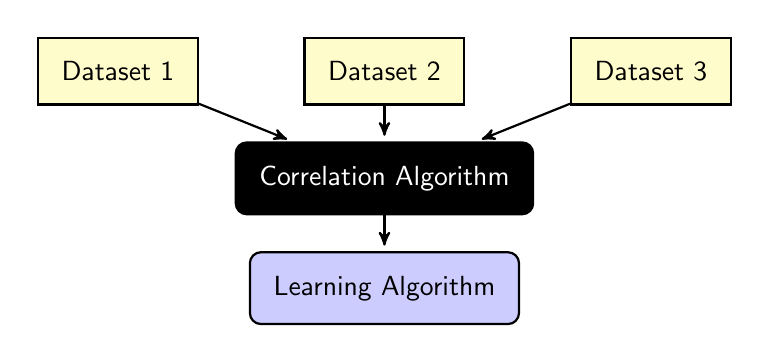
\begin{tikzpicture}[
      font=\sffamily,
      every matrix/.style={ampersand replacement=\&,column sep=3ex,row sep=3ex},
      dataset/.style={draw,thick,fill=yellow!20,inner sep=.3cm},
      sink/.style={dataset,rounded corners,fill=black, text=white},
      app/.style={dataset,rounded corners,fill=blue!20},
      dots/.style={gray,scale=2},
      to/.style={->,>=stealth',shorten >=2pt,thick,font=\sffamily\footnotesize},
      every node/.style={align=center}]

      \matrix{
        \node[dataset] (dataset1) {Dataset 1};
        \& \node[dataset] (dataset2) {Dataset 2};
        \& \node[dataset] (dataset3) {Dataset 3}; \\

        \& \node[sink] (blackbox) {Correlation Algorithm}; \& \\

        \& \node[app] (application) {Learning Algorithm}; \& \\      
      };

      \draw[to] (dataset1) -- (blackbox);
      \draw[to] (dataset2) -- (blackbox);
      \draw[to] (dataset3) -- (blackbox);
      \draw[to] (blackbox) -- (application);

    \end{tikzpicture}
  \end{center}

  \begin{center}
    \textbf{Thesis Goal}\\
    \vspace{1ex}
    \fcolorbox{black}[HTML]{F1F1F1}{\parbox{0.6\textwidth}{%
        \centering Develop theoretically justified, robust\\ correlation algorithms for\\
        multi-dataset fusion}}
  \end{center}

    
\end{frame}

\begin{frame}{A Myriad of Applications}

  \begin{columns}[T]
    \begin{column}{0.45\textwidth}
      
      \vspace{3ex}

      \textbf{Multiple Datasets}
      \begin{itemize}
      \item \textcolor<1>{texthigh}{Audio-Video}
      \item \textcolor<2>{texthigh}{Audio-Audio}
      \end{itemize}

      \hspace{2ex}
      

      \textbf{Machine learning}
      \begin{itemize}
      \item \textcolor<3>{texthigh}{emotion identification}
      \item \textcolor<4>{texthigh}{shopping predictions}
      \item \textcolor<5>{texthigh}{music genre classification}
      \end{itemize}
      
      \hspace{2ex}

      \textbf{Medical analysis}
      \begin{itemize}
      \item MRI, fMRi, EEG, MEG, etc.
      \end{itemize}

      \hspace{2ex}



      \textbf{Climatology}
      \begin{itemize}
      \item sea temperature prediction
      \item tropical cyclone prediction
      \end{itemize}


    \end{column}
    \begin{column}{0.45\textwidth}
      \begin{center}
      \includegraphics<1>[width=0.6\textwidth]{figures/parking_lot.jpg}\vspace{3ex}
      \includegraphics<1>[width=0.6\textwidth]{figures/car.png}
      \includegraphics<2>[width=0.8\textwidth]{figures/burton.jpg}
      \includegraphics<3>[width=0.6\textwidth]{figures/emotion1.png}
      \includegraphics<4>[width=0.8\textwidth]{figures/amazon_books.jpg}
      \includegraphics<5>[width=0.8\textwidth]{figures/Queen-Band.jpg}

      \vspace{4ex}

      \includegraphics<1>[width=0.6\textwidth]{figures/parking_lot2.jpg}
      \includegraphics<2>[width=0.8\textwidth]{figures/umich.png}
      \includegraphics<3>[width=0.7\textwidth]{figures/speaker_audio.pdf}
      \includegraphics<4>[width=0.8\textwidth]{figures/amazon_movies.jpg}
      \onslide<5>{\fcolorbox{black}[HTML]{F1F1F1}{\parbox{0.9\textwidth}{%
        \begin{itemize}
        \item disco influences
        \item danceable grooves
        \item repetitive melodic phrasing
        \item extensive vamping
        \item minor key tonality
        \end{itemize}}}}

  \end{center}
    \end{column}
  \end{columns}


\end{frame}


%%%%%%%%%%%%%%%%%%%%%%%%%%%%%%%%%%%%%%%%%%%%%%%%%%%%%%%%%%%%%%%%%%%%%%%%%%%%%%%%%%%%%%%%%%
\begin{frame}{Canonical Correlation Analysis}

  \textbf{What is it?}
  \begin{itemize}
  \item Dimensionality reduction algorithm for exactly 2 datasets, $X,Y$
  \item Correlation coefficients, linear transformations
  \end{itemize}

  \vspace{1ex}

  \textbf{What is it not?}
  \begin{itemize}
  \item Data fusion algorithm
  \end{itemize}
 

  \vspace{1ex}

  \begin{columns}
    \begin{column}{0.35\textwidth}
      \textbf{Covariance matrices}
      \begin{itemize}
      \item $\Rxx = \E{xx^H}$
      \item $\Ryy = \E{yy^H}$
      \item $\Rxy = \E{xy^H}$
      \end{itemize}
    \end{column}
    \begin{column}{0.55\textwidth}
      \begin{center}
        \textbf{Optimization problem}
        \vspace{-1ex}
        \begin{empheq}[box={\mybluebox[5pt][5pt][boxgrey]}]{equation*}
          \begin{aligned}
            & \argmax_{w_x,w_y} &&\rho = w_x^HR_{xy}w_y\\
            & \text{subject to } && w_x^H\Rxx w_x=1\\
            &&&w_y^H\Ryy w_y = 1\\
          \end{aligned}
        \end{empheq}
     \end{center}
    \end{column}
  \end{columns}

  \vspace{1ex}

  \textbf{Variable Transformation}
  \begin{itemize}
  \item $f=\Rxx^{1/2}w_x$
  \item $g=\Ryy^{1/2}w_y$
  \end{itemize}

\end{frame}

%%%%%%%%%%%%%%%%%%%%%%%%%%%%%%%%%%%%%%%%%%%%%%%%%%%%%%%%%%%%%%%%%%%%%%%%%%%%%%%%%%%%%%%%%%
\begin{frame}{Canonical Correlation Analysis}
  \addtocounter{framenumber}{-1}
  \textbf{What is it?}
  \begin{itemize}
  \item Dimensionality reduction algorithm for exactly 2 datasets
  \item Correlation coefficients, linear transformations
  \end{itemize}

  \vspace{1ex}

  \textbf{What is it not?}
  \begin{itemize}
  \item Data fusion algorithm
  \end{itemize}
 

  \vspace{1ex}

  \begin{center}
    \textbf{Optimization problem}
    \vspace{-1ex}
    \begin{empheq}[box={\mybluebox[5pt][5pt][boxgrey]}]{equation*}
      \begin{aligned}
        & \argmax_{f,g} &&\rho = f^H\,\underbrace{R_{xx}^{-1/2}R_{xy}R_{yy}^{-1/2}}_{\Ccca}g\\
        & \text{subject to } && \|f\|_2=1\,,\,\|g\|_2=1\\
      \end{aligned}
    \end{empheq}
  \end{center}


  \vspace{3ex}

  \begin{columns}[t]
    \begin{column}{0.3\textwidth}
      \textbf{Canonical Vectors}
      \begin{itemize}
      \item $w_x = R_{xx}^{-1/2}f$
      \item $w_y = R_{yy}^{-1/2}g$
      \end{itemize}
    \end{column}
    \begin{column}{0.4\textwidth}
      \centering
      \textbf{Insight}\\[-3ex]
      \begin{empheq}[box={\mybluebox[5pt][5pt][boxgrey]}]{equation*}
        \text{\# correlated signals $=k=\rank(\Ccca)$}
      \end{empheq}

    \end{column}
  \end{columns}

\end{frame}

%%%%%%%%%%%%%%%%%%%%%%%%%%%%%%%%%%%%%%%%%%%%%%%%%%%%%%%%%%%%%%%%%%%%%%%%%%%%%%%%%
\begin{frame}{Empirical CCA}

  \begin{columns}[t]
    \begin{column}{0.5\textwidth}

      \textbf{Training Datasets}
      \begin{itemize}
        \itemsep=1ex
      \item $X=\left[x_1,\dots,x_n\right]$
      \item $Y=\left[y_1,\dots,y_n\right]$
      \end{itemize}
    \end{column}
    \begin{column}{0.5\textwidth}

      \textbf{Sample Covariance Matrices}
      \begin{itemize}
      \item $\Rxxhat=\frac{1}{n}XX^H$
      \item $\Ryyhat=\frac{1}{n}YY^H$
      \item $\Rxyhat=\frac{1}{n}XY^H$
      \end{itemize}
    \end{column}
  \end{columns}

  \vspace{1ex}

  \begin{center}
    \textbf{Estimate}\\
    \fcolorbox{black}[HTML]{F1F1F1}{\parbox{0.4\textwidth}{%
        \be\ba
        &\Cccahat &&= \Rxxhat^{-1/2}\Rxyhat\Ryyhat^{-1/2}\\
        &&&=\widehat{F}\widehat{K}\widehat{G}^H
        \ea\ee
      }}
  \end{center}

      \textbf{Data SVDs}
      \begin{itemize}
        \itemsep=1ex
      \item $X = \Uxhat\Sigxhat\Vxhat^H$
      \item $Y=\Uyhat\Sigyhat\Vyhat^H$
      \item $ \Cccahat = \Uxhat\Vxhat^H\Vyhat\Uxhat$
      \end{itemize}

\end{frame}

%%%%%%%%%%%%%%%%%%%%%%%%%%%%%%%%%%%%%%%%%%%%%%%%%%%%%%%%%%%%%%%%%%%%%%%%%%%%%%
\begin{frame}{Motivational Example -
    \href{run:/home/user/Documents/thesis_vids/flashing_setup.mp4}{Flashing Light Video}}

  \begin{center}\textbf{Left Camera} \hspace{20ex} \textbf{Right Camera}\\
    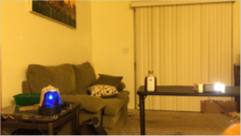
\includegraphics[width=0.47\textwidth]{figures/flashing_left.png}\hspace{2ex}
    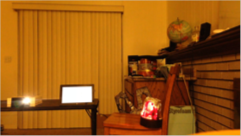
\includegraphics[width=0.47\textwidth]{figures/flashing_right.png}
  \end{center}

  \vspace{2ex}

  \textbf{System parameters}
  \begin{itemize}
  \item Vectorize $135\times 240$ image $\Rightarrow p=q=32400$ pixels
  \item 30 fps @ 30 seconds $\Rightarrow n=900$ frames
  \end{itemize}

  \begin{center}
  \textbf{Goal}\\
  \fcolorbox{black}[HTML]{F1F1F1}{\parbox{0.4\textwidth}{%
      \centering
      Identify correlated pixels between camera views
}}
\end{center}
  

\end{frame}

%%%%%%%%%%%%%%%%%%%%%%%%%%%%%%%%%%%%%%%%%%%%%%%%%%%%%%%%%%%%%%%%%%%%%%%%%%%%%%
\begin{frame}{\href{run:/home/user/Documents/thesis_vids/flashing_cca.mp4}{CCA Results} -
    Canonical Correlations}


    \begin{center}
      \textbf{Top Canonical Correlations }\\
      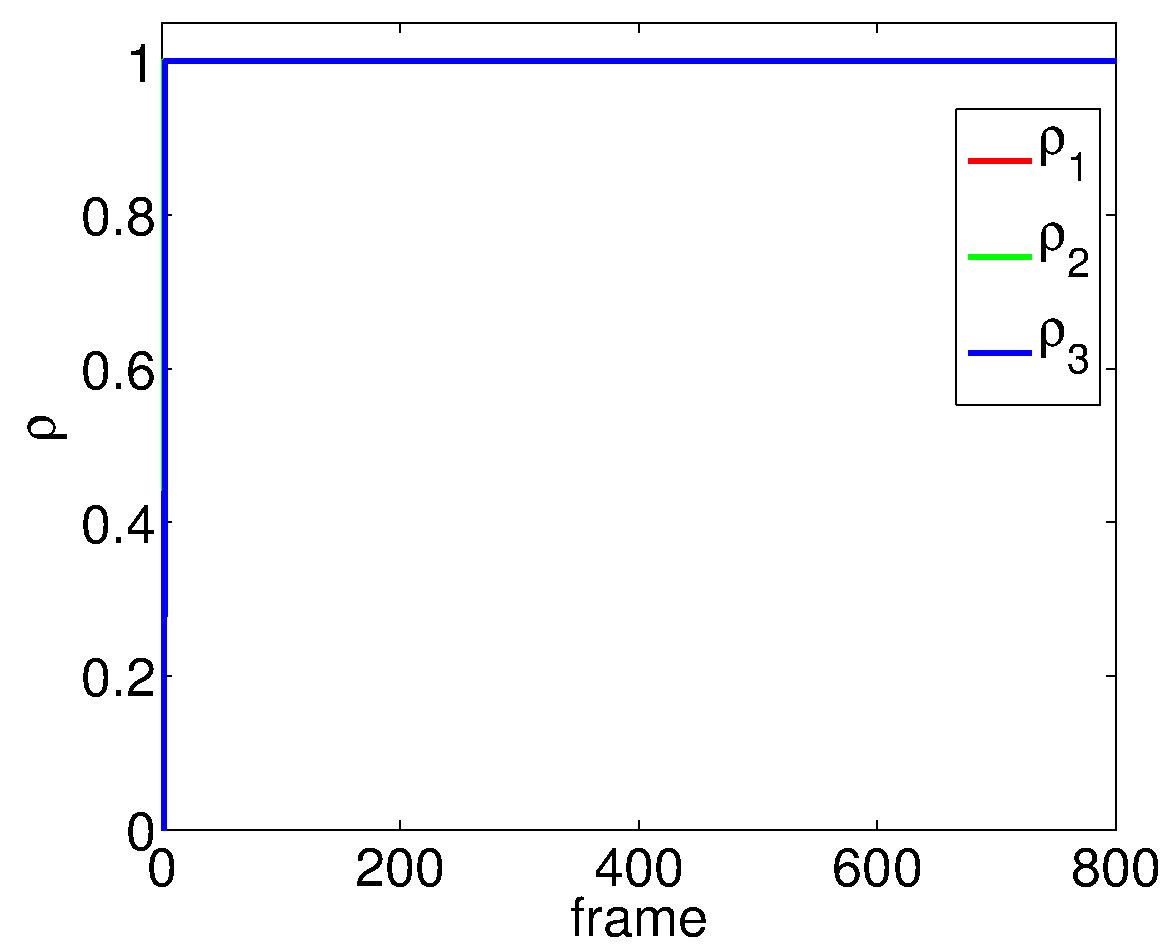
\includegraphics[width=0.5\textwidth]{figures/flashing_cca_corrs.pdf}
    \end{center}


\end{frame}

%%%%%%%%%%%%%%%%%%%%%%%%%%%%%%%%%%%%%%%%%%%%%%%%%%%%%%%%%%%%%%%%%%%%%%%%%%%%%%
\begin{frame}{\href{run:/home/user/Documents/thesis_vids/flashing_cca.mp4}{CCA Results} -
    Canonical Vectors}

  \begin{itemize}
  \item After 900 frames = 30 seconds of video  
  \end{itemize}

  \begin{columns}
    \begin{column}{0.1\textwidth}
      \textbf{Left}\\
      \vspace{15ex}
      \textbf{Right}\\
    \end{column}
    \begin{column}{0.9\textwidth}
      \begin{center}
        \textbf{First} \hspace{15ex} \textbf{Second}\hspace{15ex}\textbf{Third}\\[1ex]
        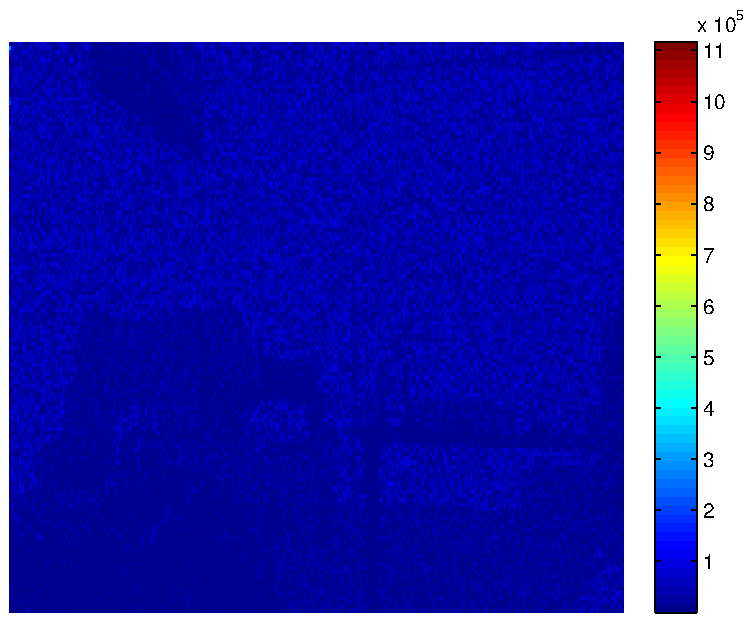
\includegraphics[width=0.3\textwidth]{figures/flashing_cca_wx1.pdf}\hspace{1ex}
        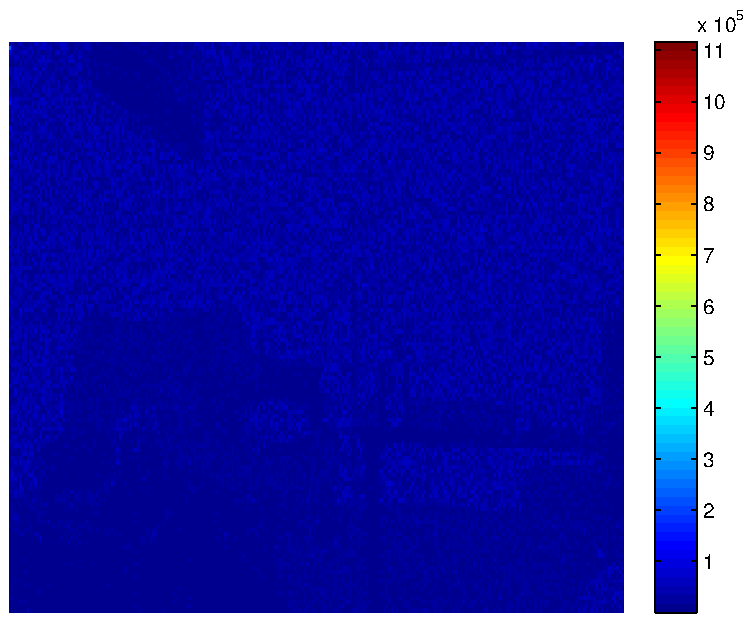
\includegraphics[width=0.3\textwidth]{figures/flashing_cca_wx2.pdf}\hspace{1ex}
        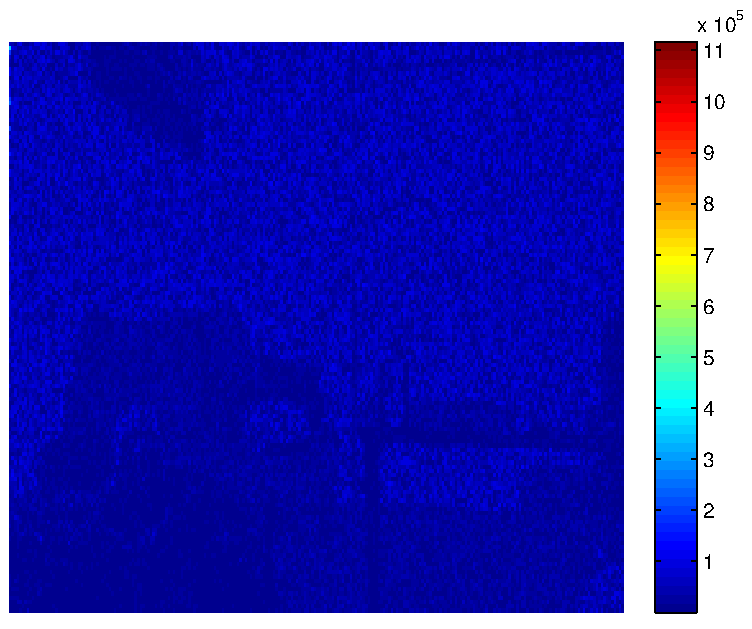
\includegraphics[width=0.3\textwidth]{figures/flashing_cca_wx3.pdf}\\[2ex]
        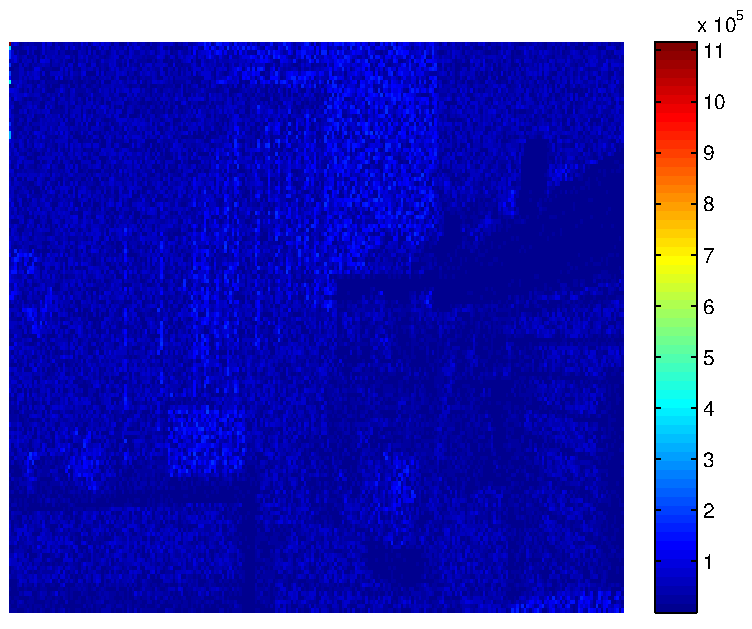
\includegraphics[width=0.3\textwidth]{figures/flashing_cca_wy1.pdf}\hspace{1ex}
        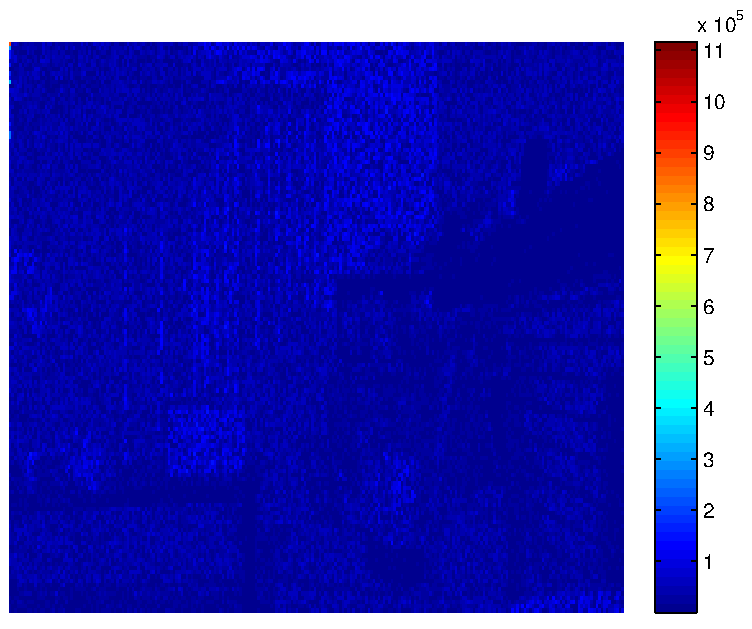
\includegraphics[width=0.3\textwidth]{figures/flashing_cca_wy2.pdf}\hspace{1ex}
        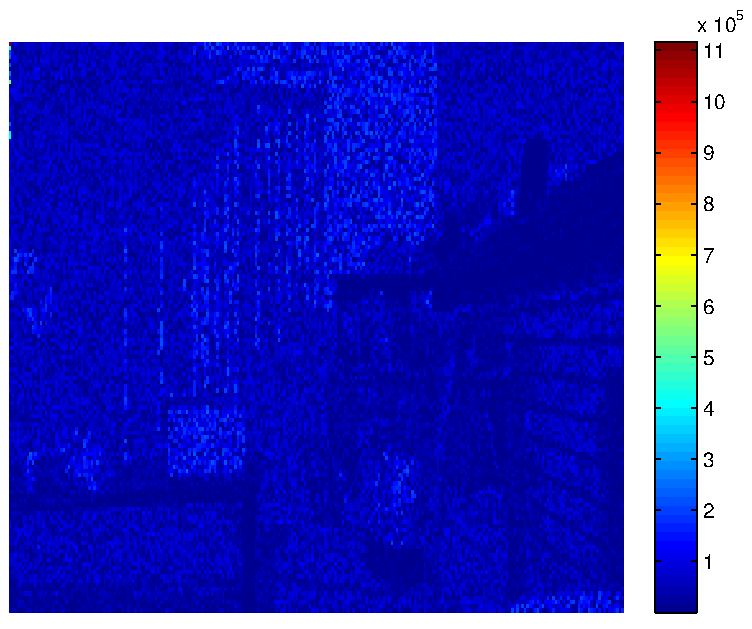
\includegraphics[width=0.3\textwidth]{figures/flashing_cca_wy3.pdf}
      \end{center}
    \end{column}
  \end{columns}

\end{frame}


%%%%%%%%%%%%%%%%%%%%%%%%%%%%%%%%%%%%%%%%%%%%%%%%%%%%%%%%%%%%%%%%%%%%%%%%%%%%%%
\begin{frame}{Previous Observations}

\centering
\fcolorbox{black}[HTML]{F1F1F1}{\parbox{0.8\textwidth}{%
    ``Therefore, the \textcolor{textred}{empirical canonical correlations are defective and
      may not be used} as     estimates of canonical correlations between random
    variables.''
    \begin{flushright}- A. Pezeshki,     L.L. Scharf et al. \\Asilomar Conference on
      Signals Systems and Computer, 2004\end{flushright}

      }}

\vspace{4ex}

\fcolorbox{black}[HTML]{F1F1F1}{\parbox{0.8\textwidth}{%
    ``In conclusion, CCA provide(s) \textcolor{textred}{reliable information} about spatial
    correlations existing among pairs of data sets \textcolor{textred}{only when SNRs ... are
    reasonably high, and the sample support is significantly larger than the data
    dimensions.}''
  \begin{flushright} - H. Ge et al. \\ICASSP, 2009 \end{flushright}}}

\end{frame}

%%%%%%%%%%%%%%%%%%%%%%%%%%%%%%%%%%%%%%%%%%%%%%%%%%%%%%%%%%%%%%%%%%%%%%%%%%%%%%
\begin{frame}{Correlation Analysis Wish List}

  \begin{center}
    \textbf{Correlation Algorithm Wish List}\\[1ex]
\fcolorbox{black}[HTML]{F1F1F1}{\parbox{0.8\textwidth}{%
    \begin{enumerate}
    \item \textbf{Works in the sample deficient regime}
      \begin{itemize}
      \item meaningful correlations
      \item meaningful canonical vectors
      \end{itemize}
    \item \textbf{Statistical test for correlations}
      \begin{itemize}
      \item consistency results
      \end{itemize}
    \item \textbf{Robustness}
      \begin{itemize}
      \item non-gaussian data
      \item missing data
      \end{itemize}
    \item \textbf{Extension to more than 2 datasets}
    \item \textbf{Unification of performance analysis}
    \end{enumerate}
}}
\end{center}

\end{frame}


%%%%%%%%%%%%%%%%%%%%%%%%%%%%%%%%%%%%%%%%%%%%%%%%%%%%%%%%%%%%%%%%%%%
\begin{frame}{Thesis Outline}

  \begin{enumerate}
  \item Introduction
  \item Performance of Matched Subspace Detectors Using Finite Training Data
  \item Extensions of Deterministic MSD to Missing Data and Useful Subspace Components
  \item Using CCA and ICCA to Detect Correlations in Low-Rank Signal-Plus-Noise Datasets
  \item On Estimating Population Canonical Vectors
  \item The Top Singular Values of $XY^H$
  \item The Largest Singular Values of a Random Projection of a Low-Rank Perturbation of a
    Random Matrix
  \item CCA and ICCA for Regression and Detection
  \item Content Based Image Retrieval and Automatic Image Annotation Using Correlations Methods
  \item Multiset CCA (MCCA)
  \end{enumerate}

\end{frame}

%%%%%%%%%%%%%%%%%%%%%%%%%%%%%%%%%%%%%%%%%%%%%%%%%%%%%%%%%%%%%%%%%%%
\begin{frame}{Thesis Outline}
  \addtocounter{framenumber}{-1}
  \begin{enumerate}
  \item \textcolor{textlightgray}{Introduction}
  \item \textcolor{textlightgray}{Performance of Matched Subspace Detectors Using Finite
      Training Data} 
  \item \textcolor{textlightgray}{Extensions of Deterministic MSD to Missing Data and
      Useful Subspace Components} 
  \item {\color{texthigh}Using CCA and ICCA to Detect Correlations in Low-Rank Signal-Plus-Noise Datasets}
  \item \textcolor{textred}{On Estimating Population Canonical Vectors}
  \item \textcolor{textred}{The Top Singular Values of $XY^H$}
  \item \textcolor{textred}{The Largest Singular Values of a Random Projection of a Low-Rank Perturbation of a Random Matrix} 
  \item \textcolor{textlightgray}{CCA and ICCA for Regression and Detection} 
  \item \textcolor{textred}{Content Based Image Retrieval and Automatic Image Annotation Using Correlations Methods}
  \item \textcolor{textred}{Multiset CCA (MCCA)}
  \end{enumerate}

\end{frame}

%%%%%%%%%%%%%%%%%%%%%%%%%%%%%%%%%%%%%%%%%%%%%%%%%%%%%%%%%%%%%%%%%%%%%%%%%%%%%%%%%%%%%%%%%%
\begin{frame}{Two-Dataset Model}

  \begin{center}
    \textbf{Linear Subspace Model\\}
    \vspace{0.5ex}
    \fcolorbox{black}[HTML]{F1F1F1}{\parbox{0.4\textwidth}{%
        \be\ba
        & x_i = \Ux\sx+\zx\\
        & y_i = \Uy\sy+\zy\\
        \ea\ee
      }}
  \end{center}

  \textbf{Parameters}
  \begin{itemize}
  \item $\Ux^H\Ux = I_{\kx}$, $\Uy^H\Uy = I_{\ky}$
  \item $\zx\simiid\mathcal{CN}(0,I_p)$, \,\,\,$\zy\simiid\mathcal{CN}(0,I_q)$
  \item
    $\E{\left[\begin{array}{c}\sx\\ \sy\end{array}\right]\left[\begin{array}{cc} \sx^H
          & \sy^H \end{array}\right]}= \left[\begin{array}{cc}\Tx & \Kxy\\
        \Kxy^H & \Ty \end{array}\right]$
  \item $\Kxy = \Tx^{1/2}\Pxy\Ty^{1/2}$
  \item $\Theta_x =
    \diag\left(\left(\theta_1^{(x)}\right)^2,\dots,\left(\theta_{k_x}^{(x)}\right)^2\right)$,\,\,\,
    $\Theta_y    =
    \diag\left(\left(\theta_1^{(y)}\right)^2,\dots,\left(\theta_{k_y}^{(y)}\right)^2\right)$  
  \item $\Pxy$ contains correlations $\rho_{kj}$ between signals of $\xii$ and $\yii$
  \item $\widetilde{K}_{xy}
    =\left(\Theta_x+I_{k_x}\right)^{-1/2}K_{xy}\left(\Theta_y+I_{k_y}\right)^{-1/2}$, with
    singular values $\kappa_1,\dots,\kappa_{\min(k_x,k_y)}$
  \end{itemize}
\end{frame}

%%%%%%%%%%%%%%%%%%%%%%%%%%%%%%%%%%%%%%%%%%%%%%%%%%%%%%%%%%%%%%%%%%%%%%%%%%%%%%%%%%%%%%%%%%
\begin{frame}{Statistical Test for CCA Correlations}

  \begin{center}
    \textbf{Estimate of \# of Correlated Signals }\\[1ex]
    \fcolorbox{black}[HTML]{F1F1F1}{\parbox{0.4\textwidth}{%
        \be
        \widehat{k}_{\text{cca}} = \sum_{i=1}^{\min(p,q)} \indicator_{\left\{\left(\widehat{\rho}_{\text{cca}}^{(i)}\right)^2 >\tau_{\text{cca}}^{\alpha}\right\}}
        \ee
      }}
  \end{center}

  \vspace{3ex}

  \begin{columns}[T]
    \begin{column}{0.6\textwidth}
      \textbf{Setting the threshold}
      \begin{itemize}
      \item $\Cccahat = \Rxxhat^{-1}\Rxyhat\Ryyhat^{-1}$ has singular values $\rhohatcca^{(i)}$
      \item $F_{\text{cca}}$ is the cdf of largest singular values of $\Cccahat$ in the
        null setting of no correlation
      \item $\tau_{\text{cca}}^{\alpha} = F_{\text{cca}}^{-1}(1-\alpha)$ 
      \item $\tau_{\text{cca}}^{\alpha} \approx \sigma_{n,p,q}\twc^{-1}(1-\alpha) + \mu_{n,p,q}$
      \end{itemize}
    \end{column}
    \begin{column}{0.4\textwidth} 
      \centering
      \textbf{Tracy-Widom Distribution}\\
      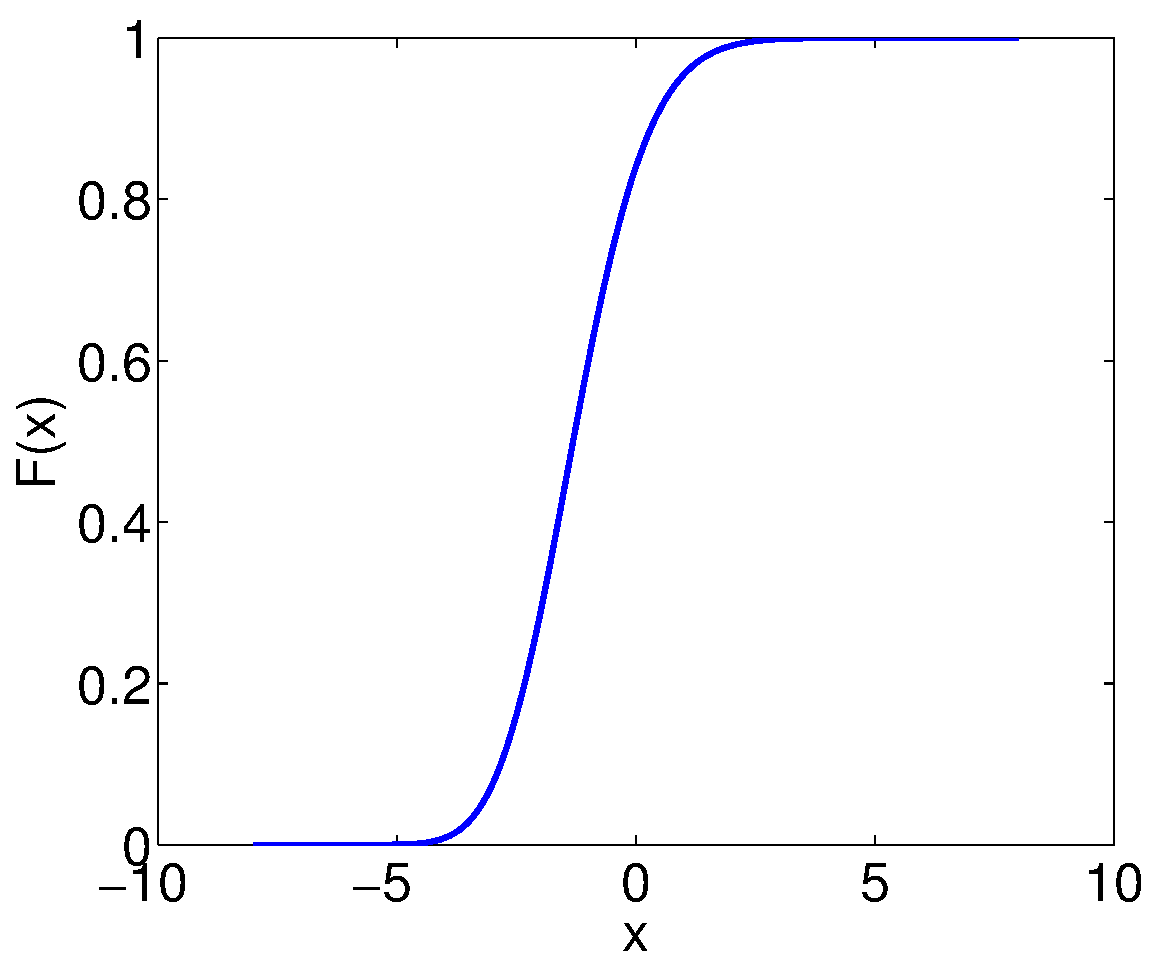
\includegraphics[width=\textwidth]{figures/tw.pdf}
    \end{column}
  \end{columns} 
\end{frame}

%%%%%%%%%%%%%%%%%%%%%%%%%%%%%%%%%%%%%%%%%%%%%%%%%%%%%%%%%%%%%%%%%%%%%%%%%%%%%%%%%%%%%%%%%%
\begin{frame}{Empirical CCA Consistency}

  \begin{Th}[Empirical CCA Consistency]\label{th:khat_lims}
    Let $p,q,n\to\infty$ with $p/n\to c_x$ and $q/n\to c_y$. Given the above linear subspace
    data model, 
    \be\ba
    & \widehat{k}_{\text{cca}} \convas k &&\text{ if } \kappa_k^2 >r_c \text{ and } n>p+q\\
    \ea\ee
    where
    \be
    r_c = \frac{c_xc_y+\sqrt{c_yc_y(1-c_x)(1-c_y)}}{(1-c_x)(1-c_y) + \sqrt{c_xc_y(1-c_x)(1-c_y)}}.
    \ee
  \end{Th}

  \vspace{3ex}

  \textbf{Recall}
  \begin{itemize}
  \item $\widetilde{K}_{xy}
    =\left(\Theta_x+I_{k_x}\right)^{-1/2}\Tx\Pxy\Ty\left(\Theta_y+I_{k_y}\right)^{-1/2}$
  \item Singular values $\kappa_1,\dots,\kappa_{\min(k_x,k_y)}$
  \end{itemize}

\end{frame}

%%%%%%%%%%%%%%%%%%%%%%%%%%%%%%%%%%%%%%%%%%%%%%%%%%%%%%%%%%%%%%%%%%%%%%%%%%%%%%%%
\begin{frame}{CCA Consistency}

  \textbf{Simulation parameters}
  \begin{itemize}
  \item $p=q=150$, $k=1$, $\theta_x=\theta_y$, $\alpha=0.01$
  \end{itemize}

  \vspace{1ex}

  \begin{center}  $\boldsymbol{\rho=}\mathbf{0.5}$\hspace{25ex}$\boldsymbol{\rho=0.9}$\\[0.5ex]
  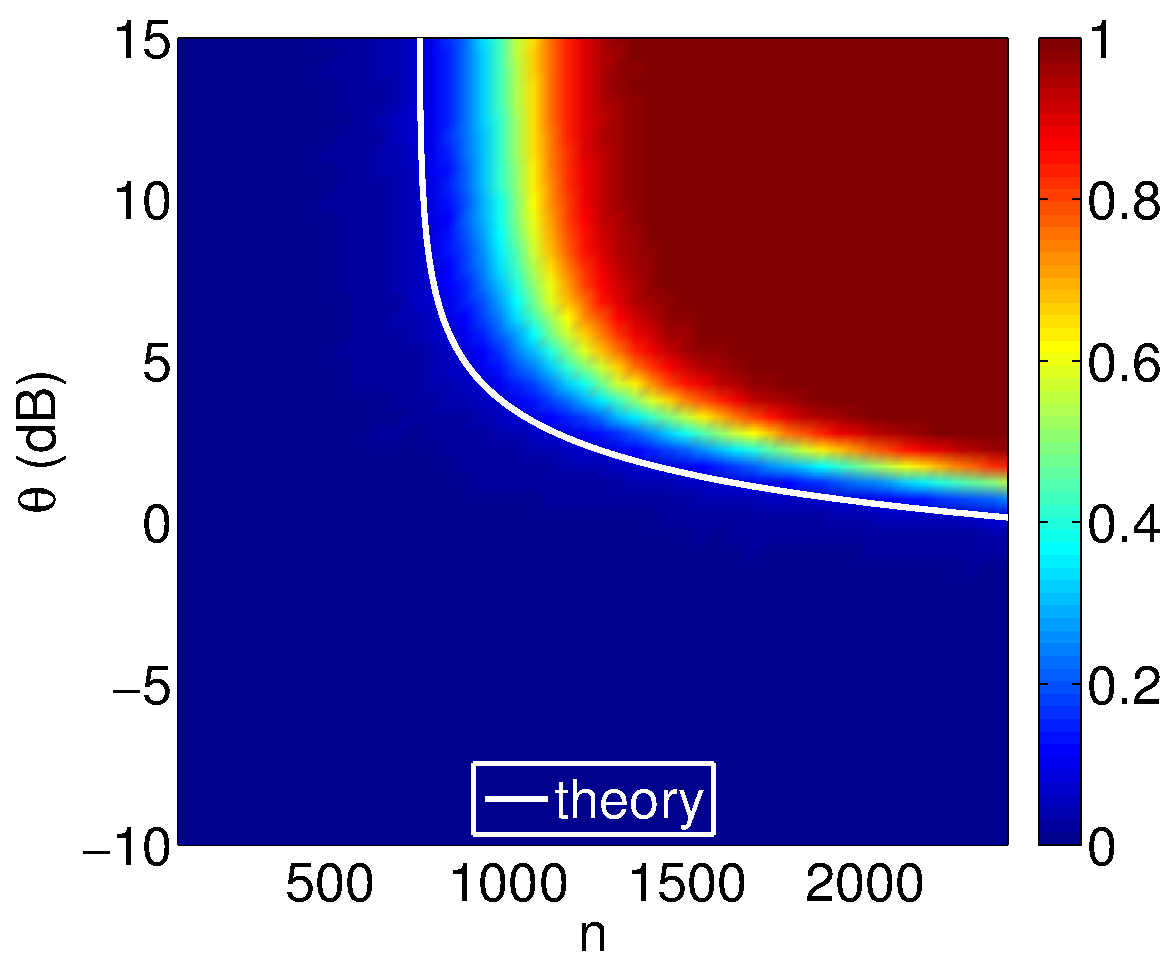
\includegraphics[width=0.4\textwidth]{figures/cca_rho5.pdf}\hspace{2ex}
  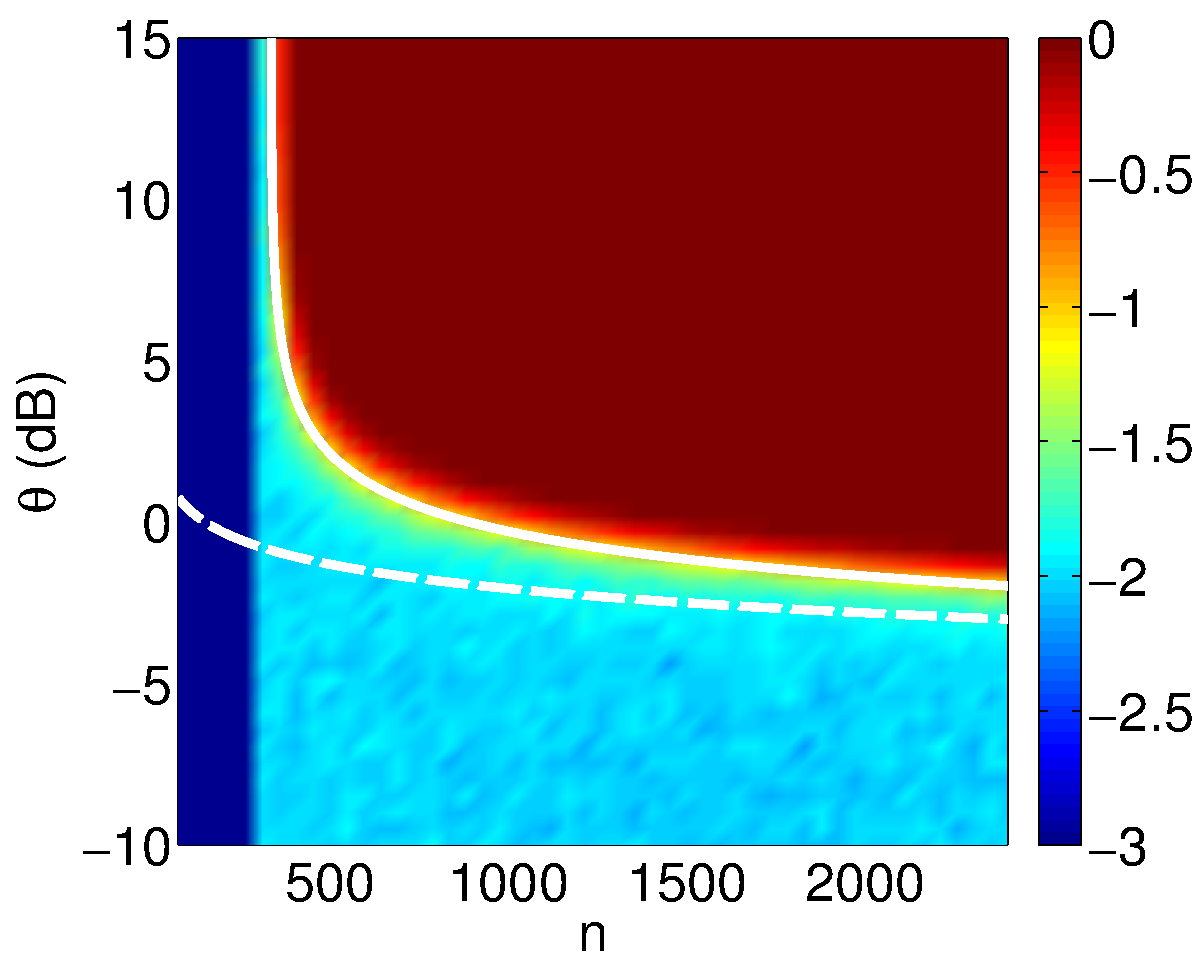
\includegraphics[width=0.4\textwidth]{figures/cca_rho9.pdf}
\end{center}



  
  \textbf{Problems!}
  \begin{itemize}
  \item Degenerate case when $n<p+q$ (Pezeshki 2004)
  \item Consistency boundary is dependent on correlation
  \end{itemize}

\end{frame}

%%%%%%%%%%%%%%%%%%%%%%%%%%%%%%%%%%%%%%%%%%%%
\begin{frame}{Informative CCA (ICCA)}

  \small

  \textbf{Not all singular vectors are informative!} (Nadakuditi, 2011)
  \begin{itemize}
  \item Trim data SVD's to only use informative components
  \end{itemize}

  \vspace{2ex}

  \fcolorbox{black}[HTML]{F1F1F1}{\parbox{0.9\textwidth}{%
  \begin{enumerate}
    \itemsep=1ex
  \item Trim data SVD's: $X=\widehat{U}_x\,\widehat{\Sigma}_x\,\widehat{V}_x^H$ and $Y=\widehat{U}_y\,\widehat{\Sigma}_y\, \widehat{V}_y^H$
    \begin{itemize}
    \item $\Uxcir = \widehat{U}_x\left(:\,,1:\widehat{k}_x\right)$, $\Uycir = \widehat{U}_y\left(:\,,1:\widehat{k}_y\right)$
    \item $\Vxcir = \widehat{V}_x\left(:\,,1:\widehat{k}_x\right)$, $\Vycir = \widehat{V}_y\left(:\,,1:\widehat{k}_y\right)$
    \end{itemize}

  \item Form
    $\Ciccahat=\Uxcir\Vxcir^H\Vycir\Uycir$
  \item Take SVD: $\Ciccahat = \widetilde{F}\widetilde{K}\widetilde{G}^H$
  \item $\widehat{\rho}_{\text{icca}}^{(i)} = \widetilde{k}_i$
  \item $\widetilde{w}_x^{(i)}=\widehat{R}_{xx}^{-1/2}\,\widetilde{f}_i$
  \item $\widetilde{w}_y^{(i)}=\widehat{R}_{yy}^{-1/2}\,\widetilde{g}_i$
  \end{enumerate}}}

\end{frame}

%%%%%%%%%%%%%%%%%%%%%%%%%%%%%%%%%%%%%%%%%%%%%%%%%%%%%%%%%%%%%%%%%%%%%%%%%%%%%%%%
\begin{frame}{Statistical Test for ICCA Correlations}


  \begin{center}
    \textbf{Estimate of \# of Correlated Signals }\\[1ex]
    \fcolorbox{black}[HTML]{F1F1F1}{\parbox{0.4\textwidth}{%
        \be
        \widehat{k}_{\text{icca}} = \sum_{i=1}^{\min(\widehat{k}_x,\widehat{k}_y)} \indicator_{\left\{\left(\widehat{\rho}_{\text{icca}}^{(i)}\right)^2 >\tau_{\text{icca}}^{\alpha}\right\}}
        \ee
      }}
  \end{center}

  \textbf{Setting the threshold}
  \begin{itemize}
  \item $F_{\text{icca}}$ is the cdf of largest singular values of $\Ciccahat$ in the null setting
    of no correlation
  \item $\tau_{\text{icca}}^{\alpha} = F_{\text{icca}}^{-1}(1-\alpha)$ 
  \item $\tau_{\text{icca}}^{\alpha} \approx \sigma_{n,\kxhat,\kyhat}\twc^{-1}(1-\alpha) + \mu_{n,\kxhat,\kyhat}$
  \end{itemize}


  \begin{Th}[ICCA Consistency]\label{th:khat_lims}
    Let $p,q,n\to\infty$ with $p/n\to c_x$ and $q/n\to c_y$. Given the linear subspace
    data model, 
    \be\ba
    & \widehat{k}_{\text{icca}} \convas k && \text{ if } \min_{i=1,\dots,k_x} \theta_i^{(x)}>c_x^{1/4} \text{ and }
    \min_{i=1,\dots,k_y} \theta_i^{(y)}>c_y^{1/4} 
    \ea\ee
  \end{Th}
\end{frame}

%%%%%%%%%%%%%%%%%%%%%%%%%%%%%%%%%%%%%%%%%%%%%%%%%%%%%%%%%%%%%%%%%%%%%%%%%%%%%%%%
\begin{frame}{CCA and ICCA Consistency}
  \begin{itemize}
  \item $p=q=150$, $k=1$, $\theta_x=\theta_y$,$\alpha=0.01$
  \end{itemize}

  \begin{columns}[T]
  \begin{column}{0.01\textwidth}
    \vspace{15ex}
    \textbf{ CCA}\\
    \vspace{20ex}
    \textbf{ICCA}
  \end{column}
  \begin{column}{1\textwidth}
    \begin{center}
      $\boldsymbol{\rho=}\mathbf{0.5}$\hspace{25ex}$\boldsymbol{\rho=0.9}$\\[0.5ex]

        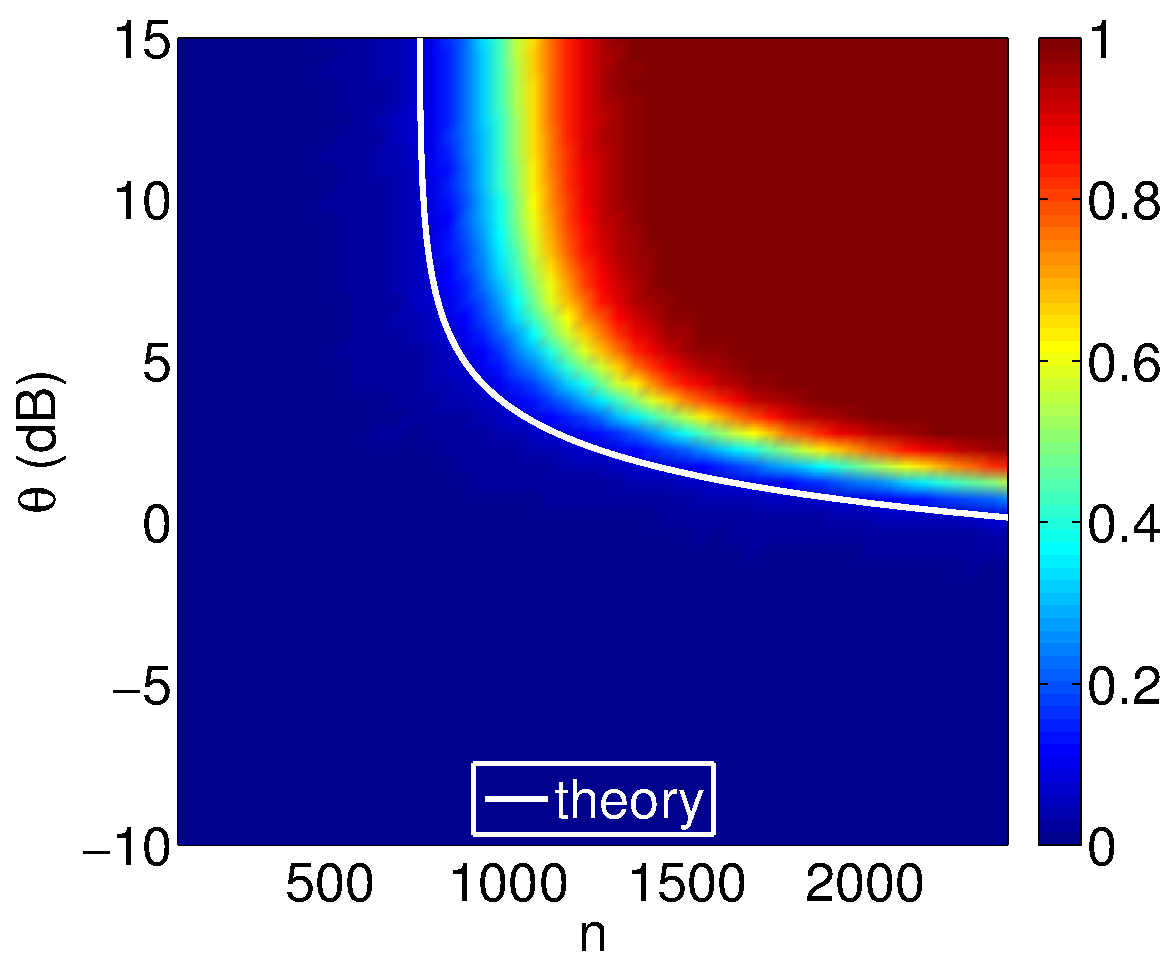
\includegraphics[width=0.35\textwidth]{figures/cca_rho5.pdf}\hspace{2ex}
        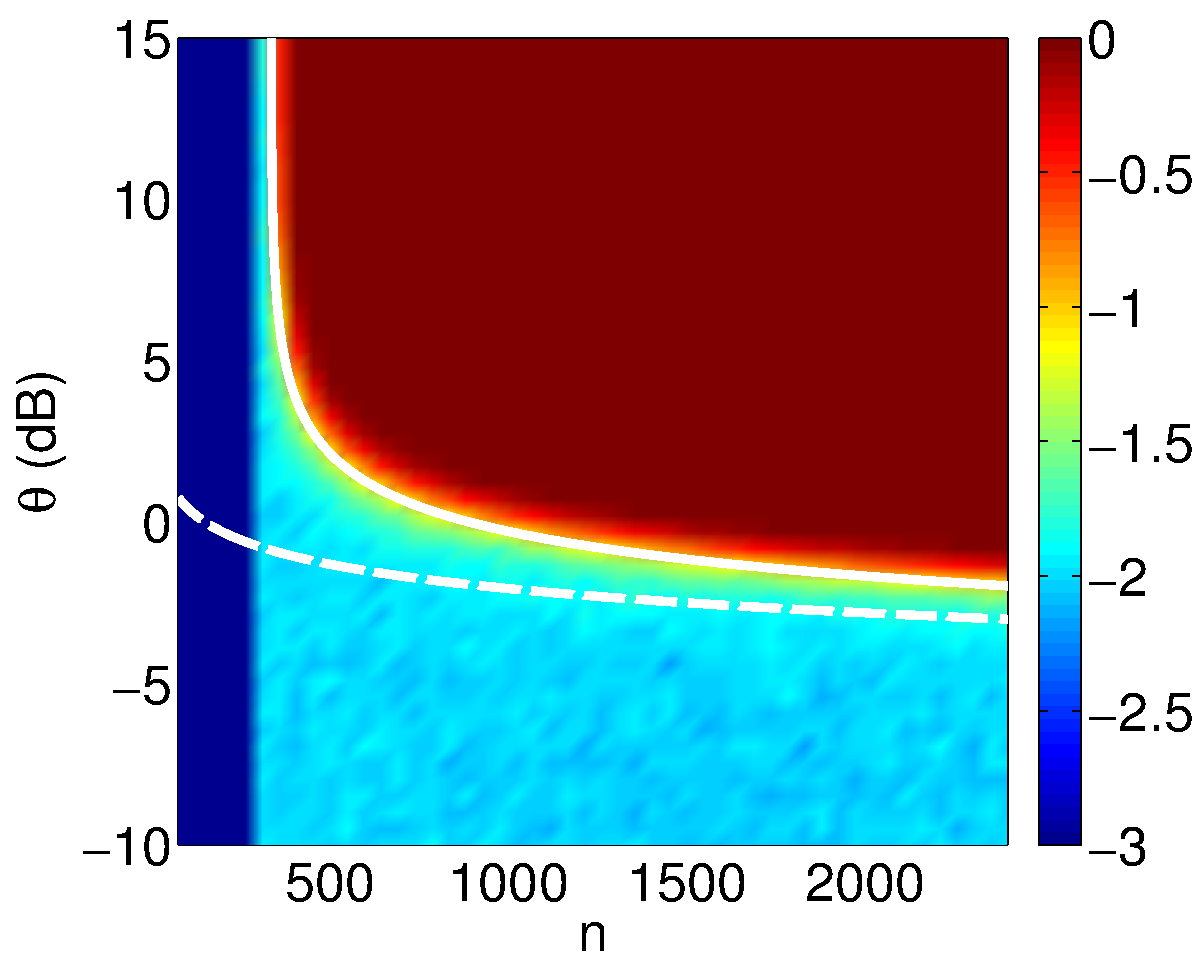
\includegraphics[width=0.35\textwidth]{figures/cca_rho9.pdf}\\[2ex]
        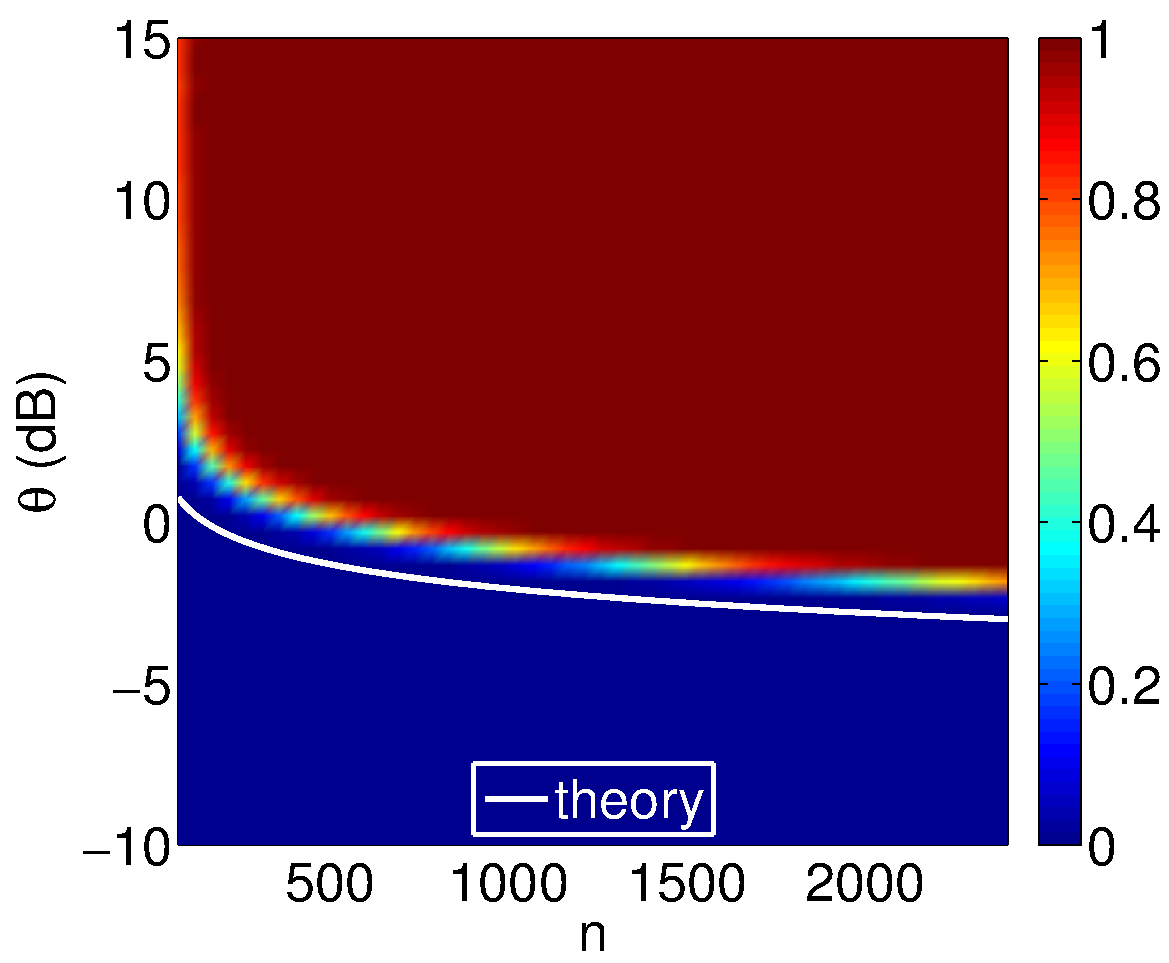
\includegraphics[width=0.35\textwidth]{figures/icca_rho5.pdf}\hspace{2ex}
        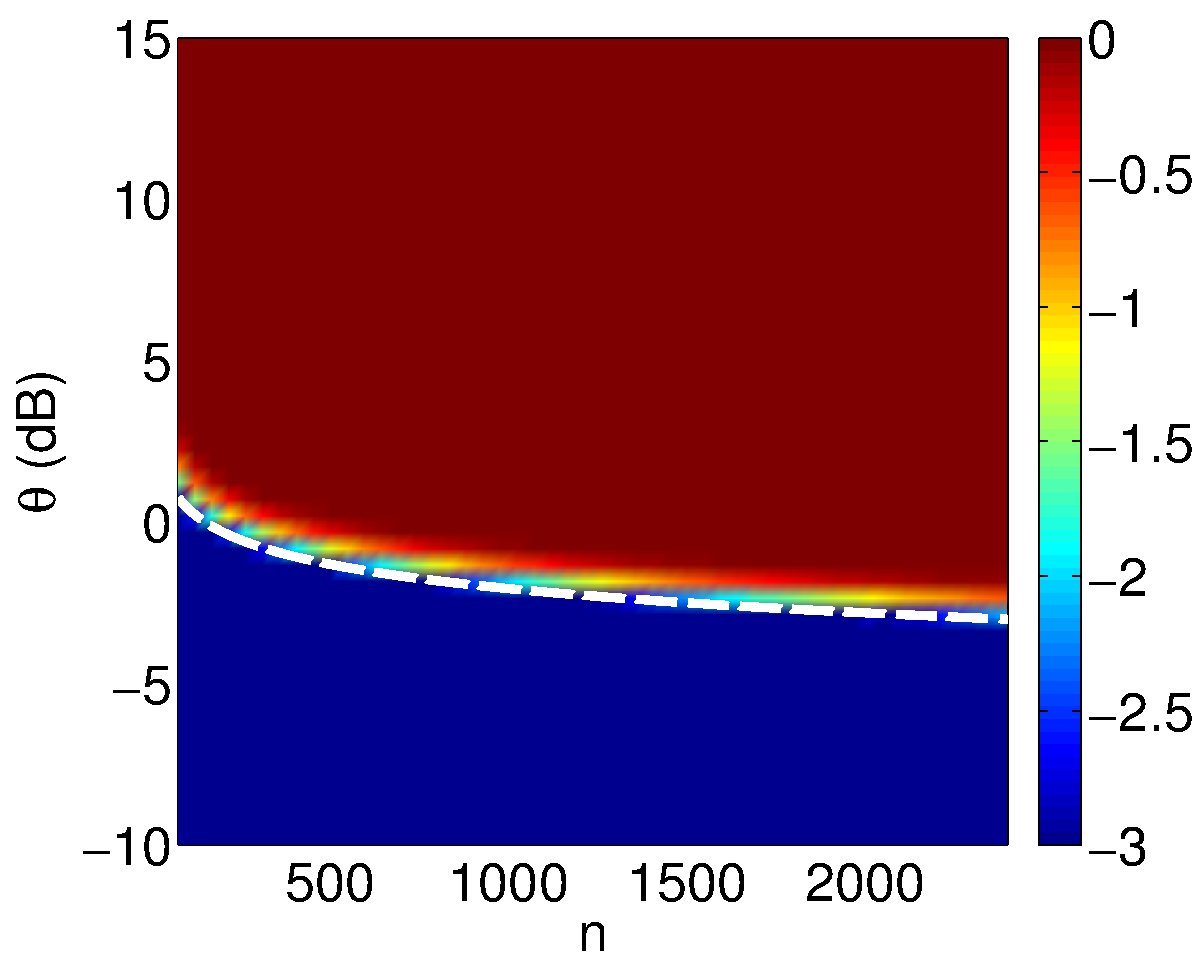
\includegraphics[width=0.35\textwidth]{figures/icca_rho9.pdf}
    \end{center}

  \end{column}
  \end{columns}



\end{frame}

%%%%%%%%%%%%%%%%%%%%%%%%%%%%%%%%%%%%%%%%%%%%%
\begin{frame}{CCA and ICCA Demonstration}
%      \textbf{ICCA Correlations}\hspace{20ex}\textbf{Significance}

  \begin{columns}[T]
  \begin{column}{0.01\textwidth}
    \vspace{15ex}
    \textbf{Correlations}\\
    \vspace{20ex}
    \textbf{Significance}
  \end{column}
  \begin{column}{1\textwidth}
    \begin{center}
      \href{run:/home/user/Documents/thesis_vids/flashing_video2.mp4}{\textbf{Video-Video}}\hspace{20ex}\href{run:/home/user/Documents/thesis_vids/av_coffee_pres.mp4}{\textbf{Audio-Video}}\\
        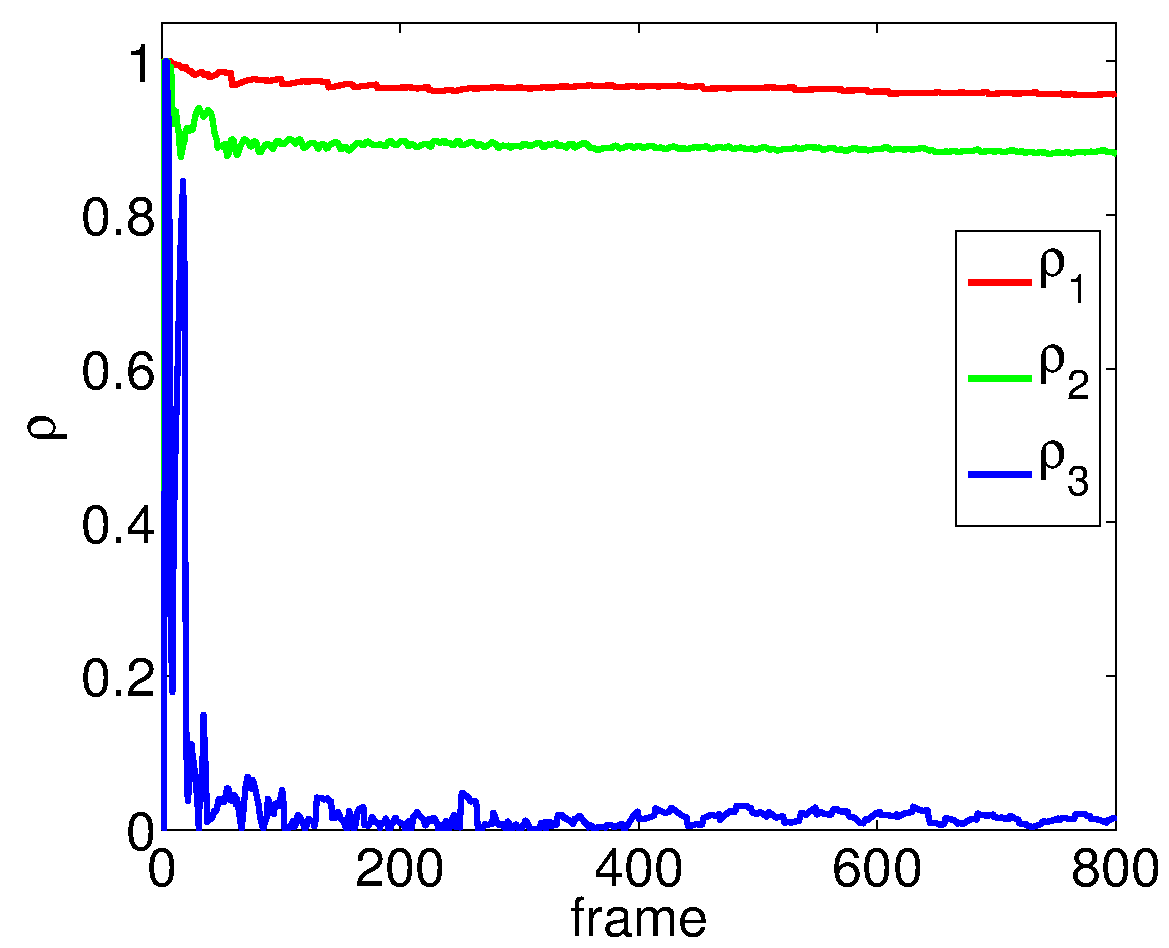
\includegraphics[width=0.38\textwidth]{figures/flashing_icca_corrs.pdf}
        \hspace{2ex}
        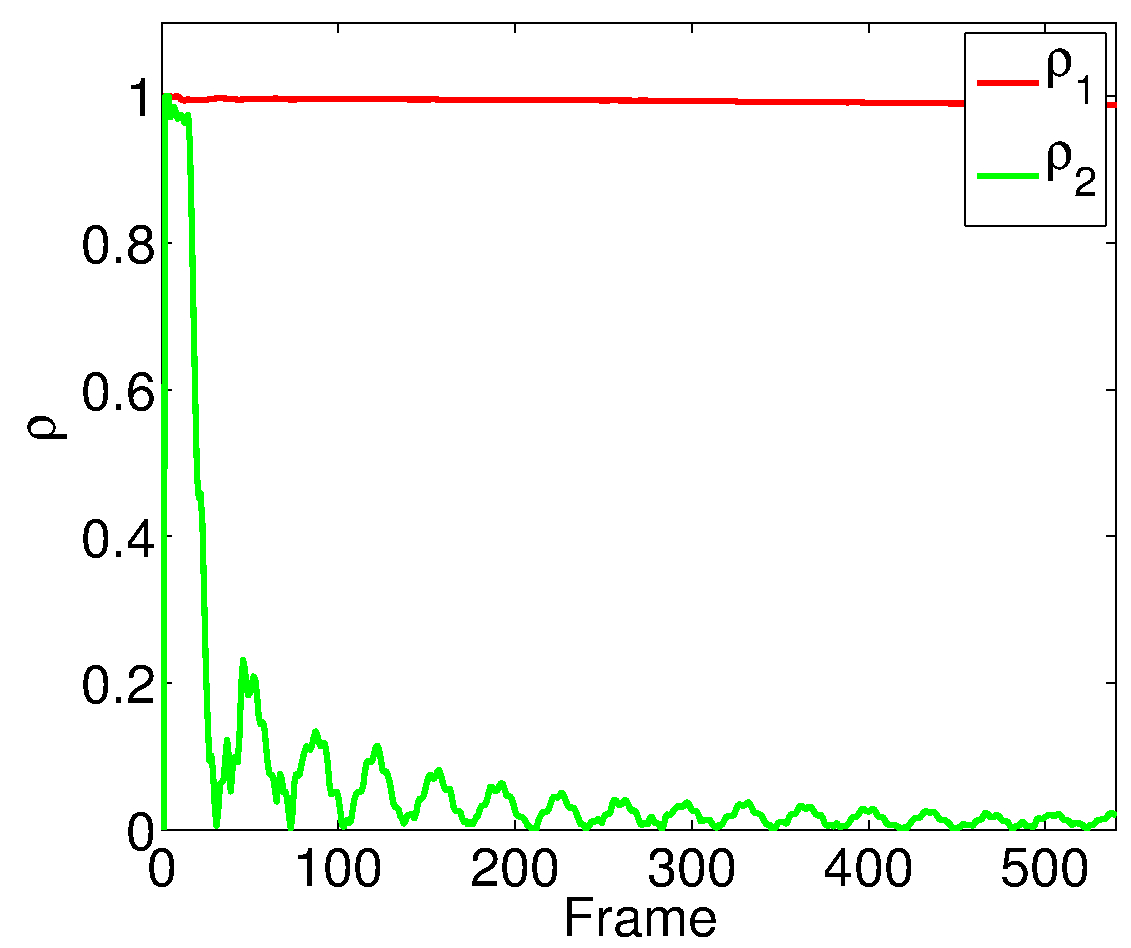
\includegraphics[width=0.38\textwidth]{figures/av_icca_corrs.pdf}\\[2ex]
        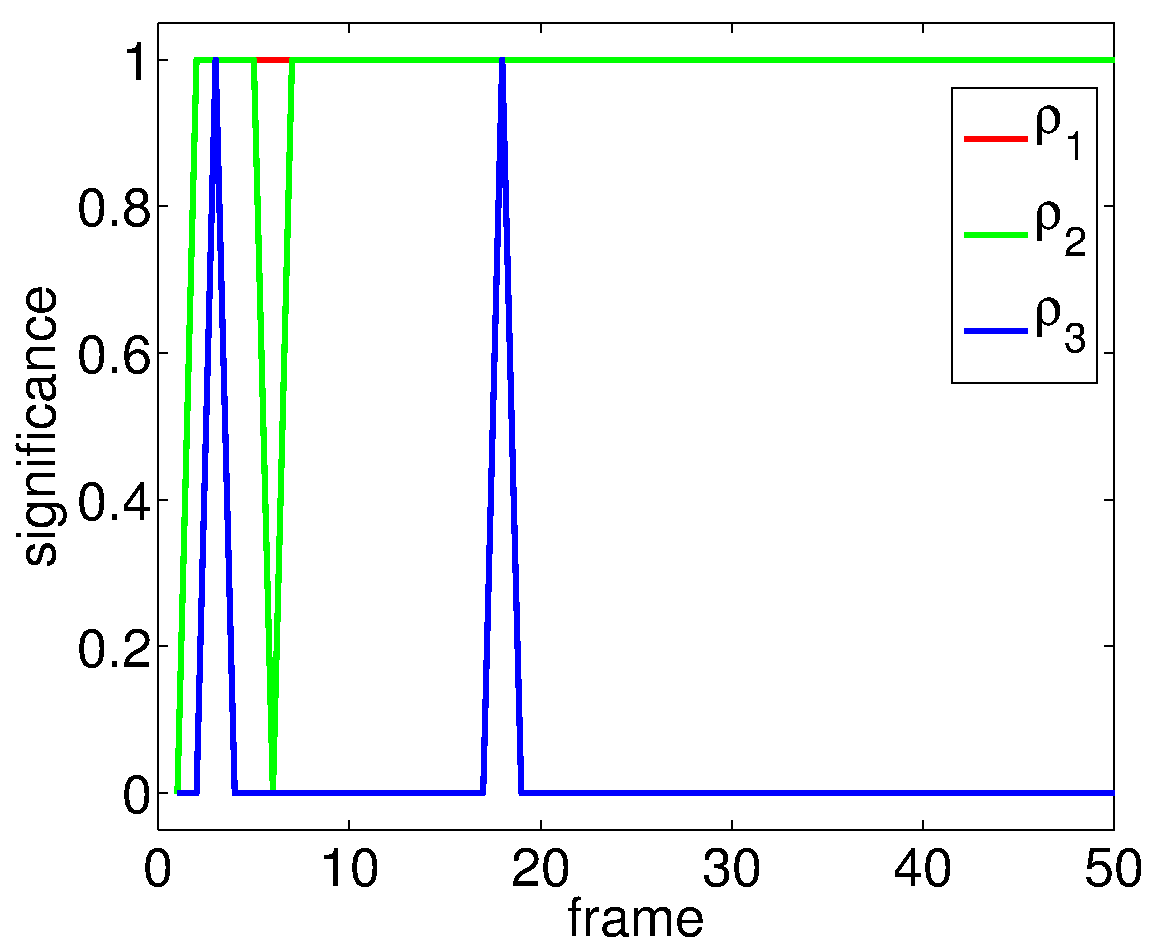
\includegraphics[width=0.38\textwidth]{figures/flashing_icca_sig_zoom.pdf}
        \hspace{2ex}
        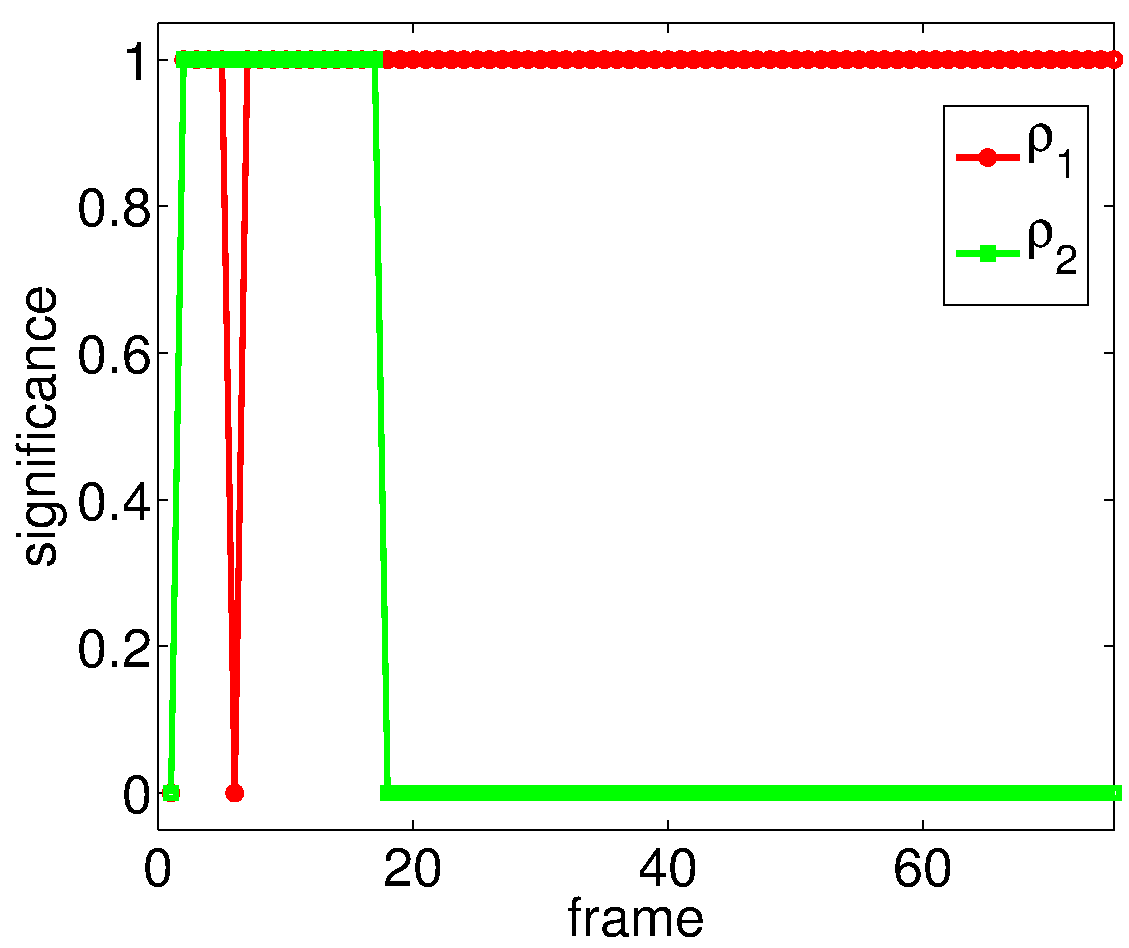
\includegraphics[width=0.38\textwidth]{figures/av_icca_sig_zoom.pdf}
    \end{center}
  \end{column}
  \end{columns}


\end{frame}

%%%%%%%%%%%%%%%%%%%%%%%%%%%%%%%%%%%%%%%%%%%%%%%%%%%%%%%%%%%%%%%%%%%%%%%%%%%%%%
\begin{frame}{Correlation Analysis Wish List}
  \addtocounter{framenumber}{-1}

  \begin{center}
    \textbf{Correlation Algorithm Wish List}\\[1ex]
\fcolorbox{black}[HTML]{F1F1F1}{\parbox{0.8\textwidth}{%
    \begin{enumerate}
    \item \textbf{Works in the sample deficient regime}
      \begin{itemize}
      \item {\textcolor{texthigh}{meaningful correlations \checkmark}}
      \item meaningful canonical vectors
      \end{itemize}
    \item {\textcolor{texthigh}{\textbf{Statistical test for correlations} \checkmark}}
      \begin{itemize}
      \item {\textcolor{texthigh}{consistency results \checkmark}}
      \end{itemize}
    \item \textbf{Robustness}
      \begin{itemize}
      \item non-gaussian data
      \item missing data
      \end{itemize}
    \item \textbf{Extension to more than 2 datasets}
    \item \textbf{Unification of performance analysis}
    \end{enumerate}
}}
\end{center}

\end{frame}

%%%%%%%%%%%%%%%%%%%%%%%%%%%%%%%%%%%%%%%%%%%%%%%%%%%%%%%%%%%%%%%%%%%%%%%%%%%%
\begin{frame}{Missing Data Model}

\textbf{Matrix model}
\begin{itemize}
\item $V_x = \left[s_{x,1},\dots,s_{x,n}\right]$, $V_y = \left[s_{y,1},\dots,s_{y,n}\right]$
\item $Z_x = \left[z_{x,1},\dots,z_{x,n}\right]$, $Z_y = \left[z_{y,1},\dots,z_{y,n}\right]$
\end{itemize}

\vspace{2ex}

\begin{center}
\fcolorbox{black}[HTML]{F1F1F1}{\parbox{0.5\textwidth}{
    \be\ba
    & X = \left(U_xV_x^H + Z_x\right)\odot M_x\\
    & Y = \left(U_yV_y^H + Z_y\right)\odot M_y\\
    \ea\ee
  }}
\end{center}

\be\ba
& M^x_{ij} = \begin{cases} 1 & \text{ with probability } \gamma_x\\ 0 & \text{ with
    probability } 1-\gamma_x \end{cases}
& M^y_{ij} = \begin{cases} 1 & \text{ with probability } \gamma_y\\ 0 & \text{ with
    probability } 1-\gamma_y \end{cases}
\ea\ee
\begin{itemize}
\item $\odot$ denotes the Hadamard or element-wise product.
\end{itemize}
\end{frame}

%%%%%%%%%%%%%%%%%%%%%%%%%%%%%%%%%%%%%%%%%%%%%%%%%%%%%%%%%%%%%%%%%%%%%%%%%%%%
\begin{frame}{CCA and ICCA Consistency in Missing Data}

\begin{Th}[Missing data consistency]\label{th:missing_data}
Let $p,q,n\to\infty$ with $p/n\to c_x$ and $q/n\to c_y$ and assume a low-coherence
condition on the signal vectors. Given a linear subspace data model with missing data
entries, 
\be\ba
& \widehat{k}_{\text{cca}} \convas k &&\text{ if } \min_{i=1,\dots,k}\kapcir_i^2 >r_c \text{ and } n>p+q\\
& \widehat{k}_{\text{icca}} \convas k && \text{ if } \min_{i=1,\dots,\widehat{k}_x}
\theta_i^{(x)}>\frac{c_x^{1/4}}{\sqrt{\gamma_x}} \text{ and } 
\min_{i=1,\dots,\widehat{k}_y} \theta_i^{(y)}>\frac{c_y^{1/4}}{\sqrt{\gamma_y}}
\ea\ee
where $\kapcir_i$ are the singular values of 
\be
\left(\gamma_x\Theta_x+I_{k_x}\right)^{-1/2}\left(\gamma_x\Theta_x\right)^{1/2}P_{xy}\left(\gamma_y\Theta_y\right)^{1/2}
\left(\gamma_y\Theta_y+I_{k_y}\right)^{-1/2}.
\ee
\end{Th}

\end{frame}

%%%%%%%%%%%%%%%%%%%%%%%%%%%%%%%%%%%%%%%%%%%%%%%%%%%%%%%%%%%%%%%%%%%%%%%%%%%%
\begin{frame}{CCA and ICCA Consistency in Missing Data}

  \begin{itemize}
  \item $p=q=150$, $k=1$, $\theta_x=\theta_y$,$\alpha=0.01$
  \end{itemize}

\setcounter{subfigure}{0}
\begin{figure}
  \begin{center}
    \subfigure[CCA $\rho=0.5$,$n=1200$]{
      \label{fig:cca_rho3_75}
      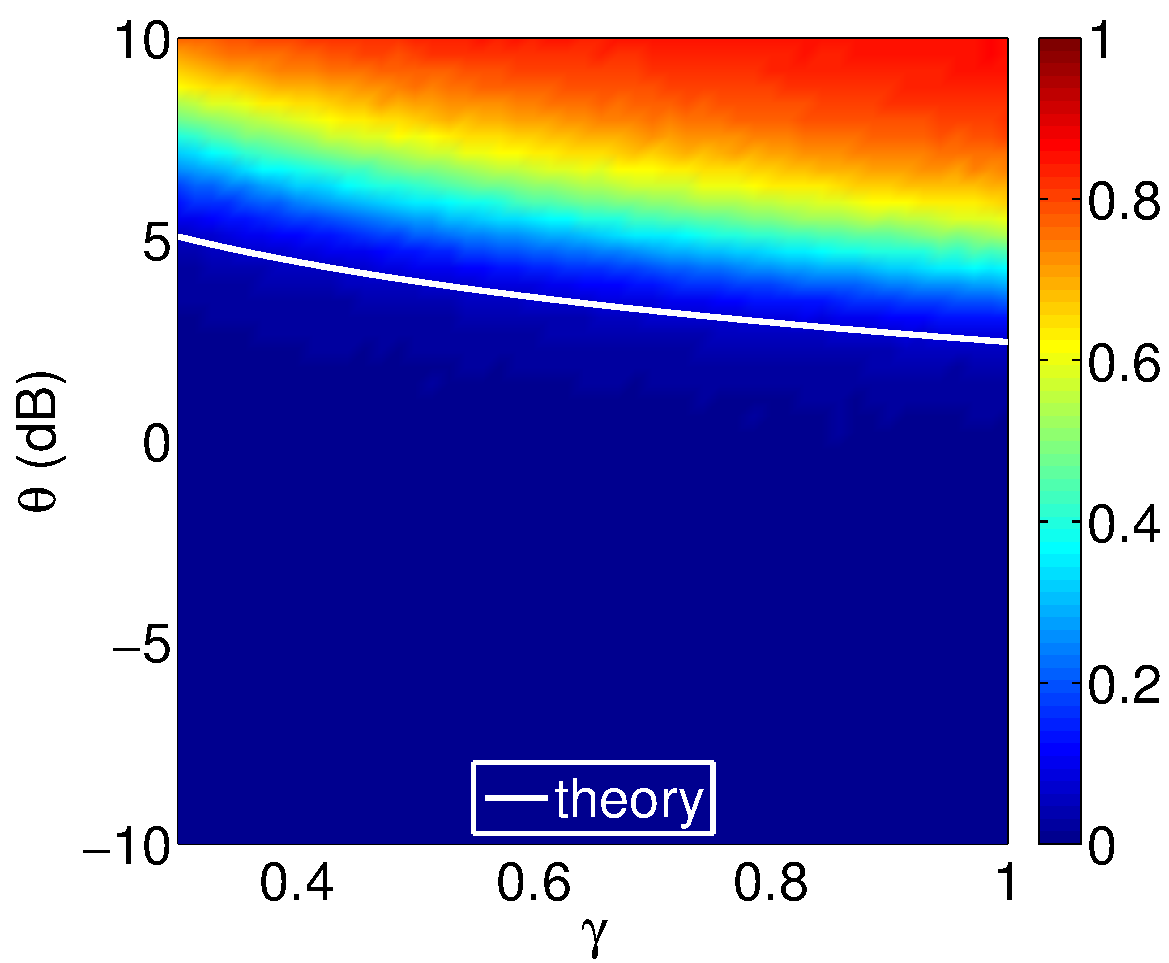
\includegraphics[width=0.35\textwidth]{figures/cca_missing_5_1200.pdf}
    }
    \subfigure[CCA $\rho=0.9$,$n=1200$]{
      \label{fig:cca_rho5_75}
      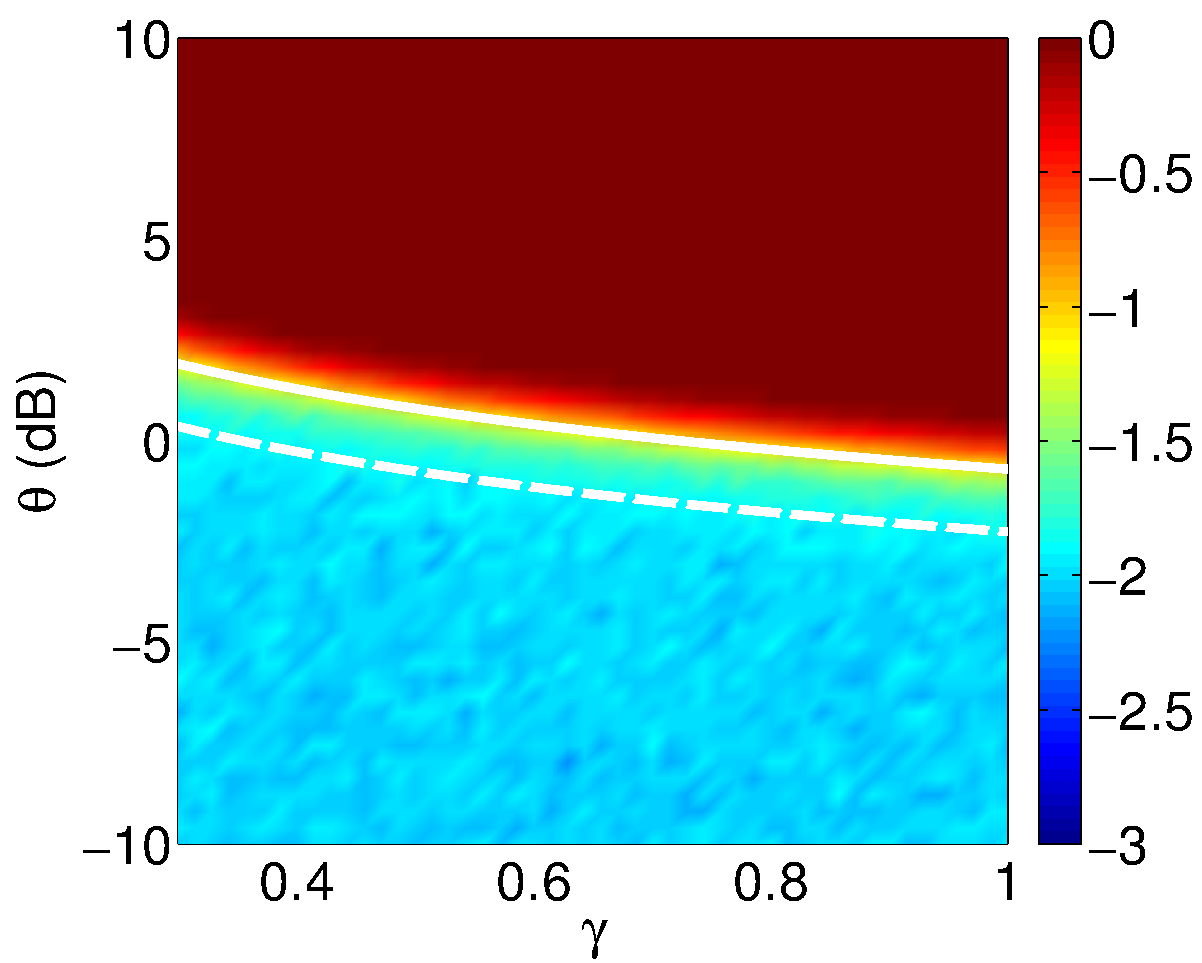
\includegraphics[width=0.35\textwidth]{figures/cca_missing_9_1200.pdf}
    }
    \subfigure[ICCA $\rho=0.5$, $n=1200$]{
      \label{fig:cca_rho7_75}
      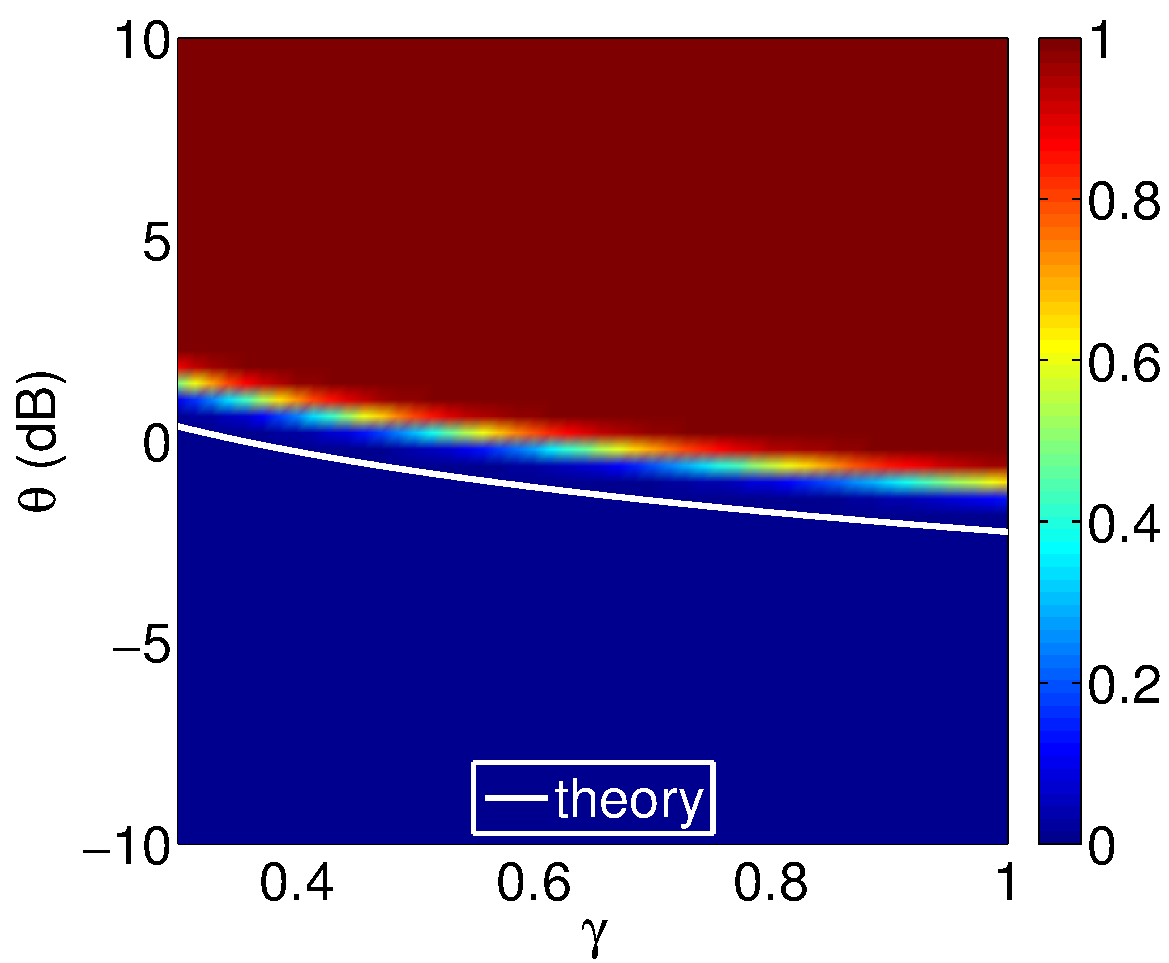
\includegraphics[width=0.35\textwidth]{figures/icca_missing_5_1200.pdf}
    }
    \subfigure[ICCA $\rho=0.9$, $n=1200$]{
      \label{fig:cca_rho9_75}
      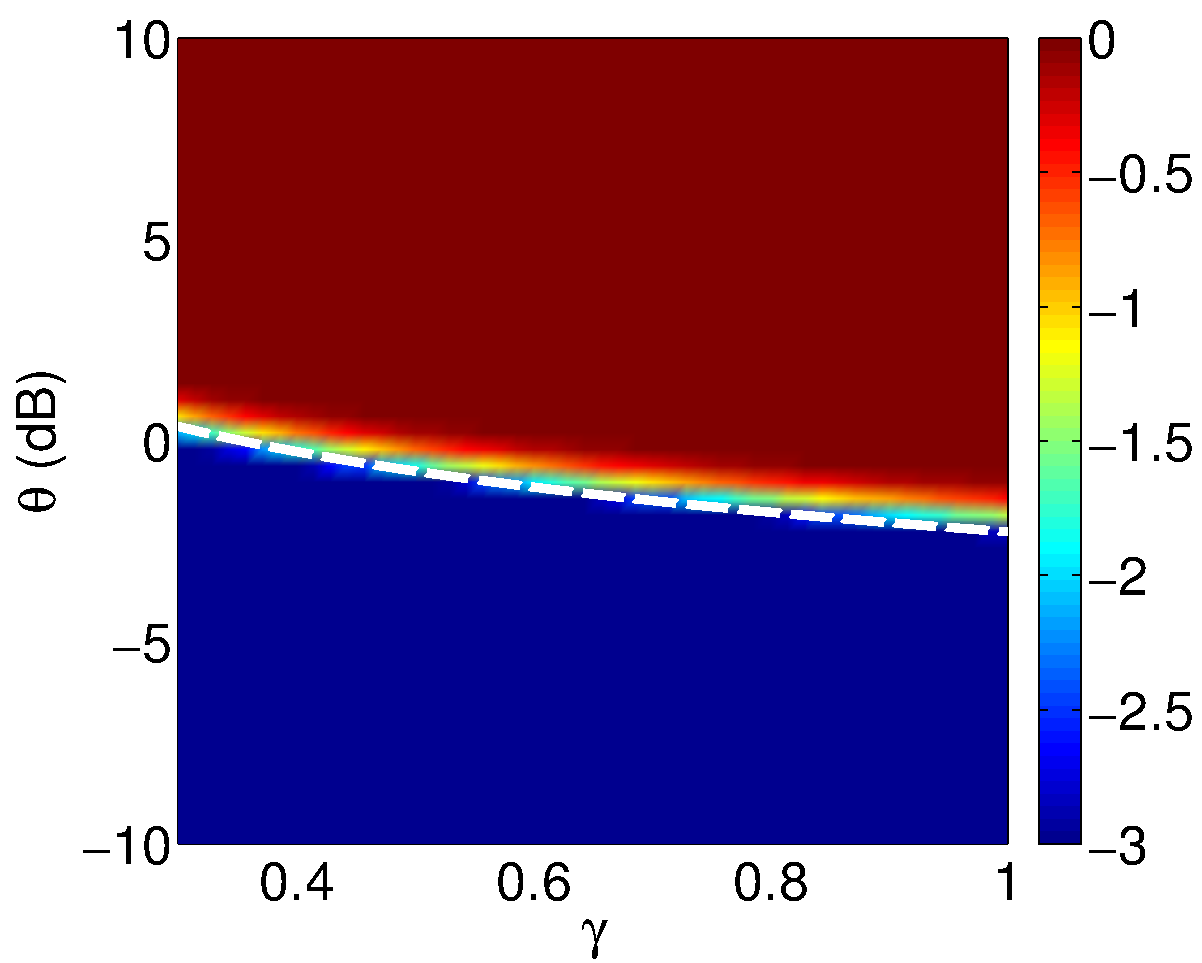
\includegraphics[width=0.35\textwidth]{figures/icca_missing_9_1200.pdf}
    }   
  \end{center}
\end{figure}

\end{frame}

%%%%%%%%%%%%%%%%%%%%%%%%%%%%%%%%%%%%%%%%%%%%%%%%%%%%%%%%%%%%%%%%%%%%%%%%%%%%%%
\begin{frame}{\href{run:/home/user/Documents/thesis_vids/youtube_missing.mp4}{Missing Data
      Demonstration}}

  \begin{itemize}
  \item $p=q=32400$ pixels
  \item $\gamma_x=\gamma_y=0.75$
  \end{itemize}

  \vspace{3ex}

  \begin{center}
    \textbf{ICCA Correlations}\hspace{23ex}\textbf{Significance}\\[0.5ex]
    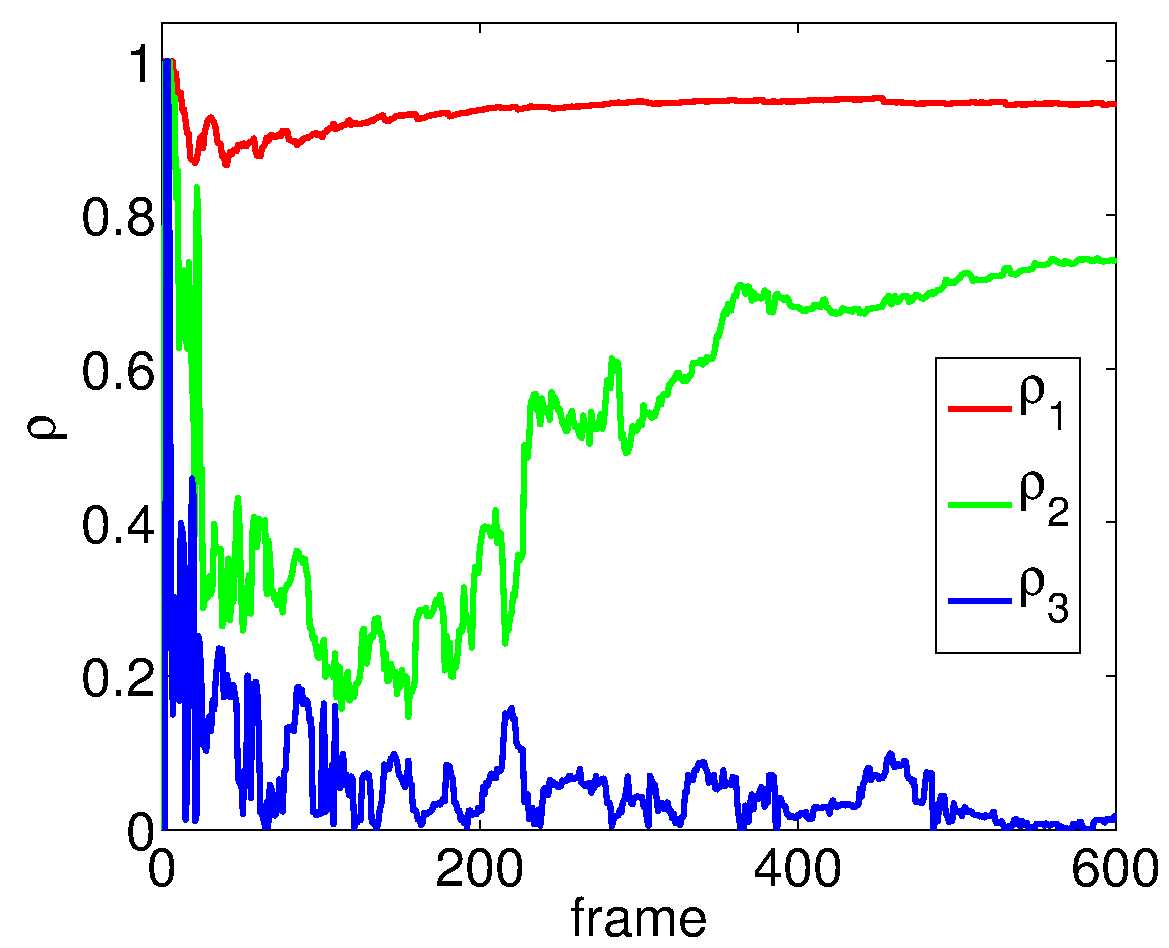
\includegraphics[width=0.45\textwidth]{figures/icca_corrs_miss.pdf}\hspace{2ex}
    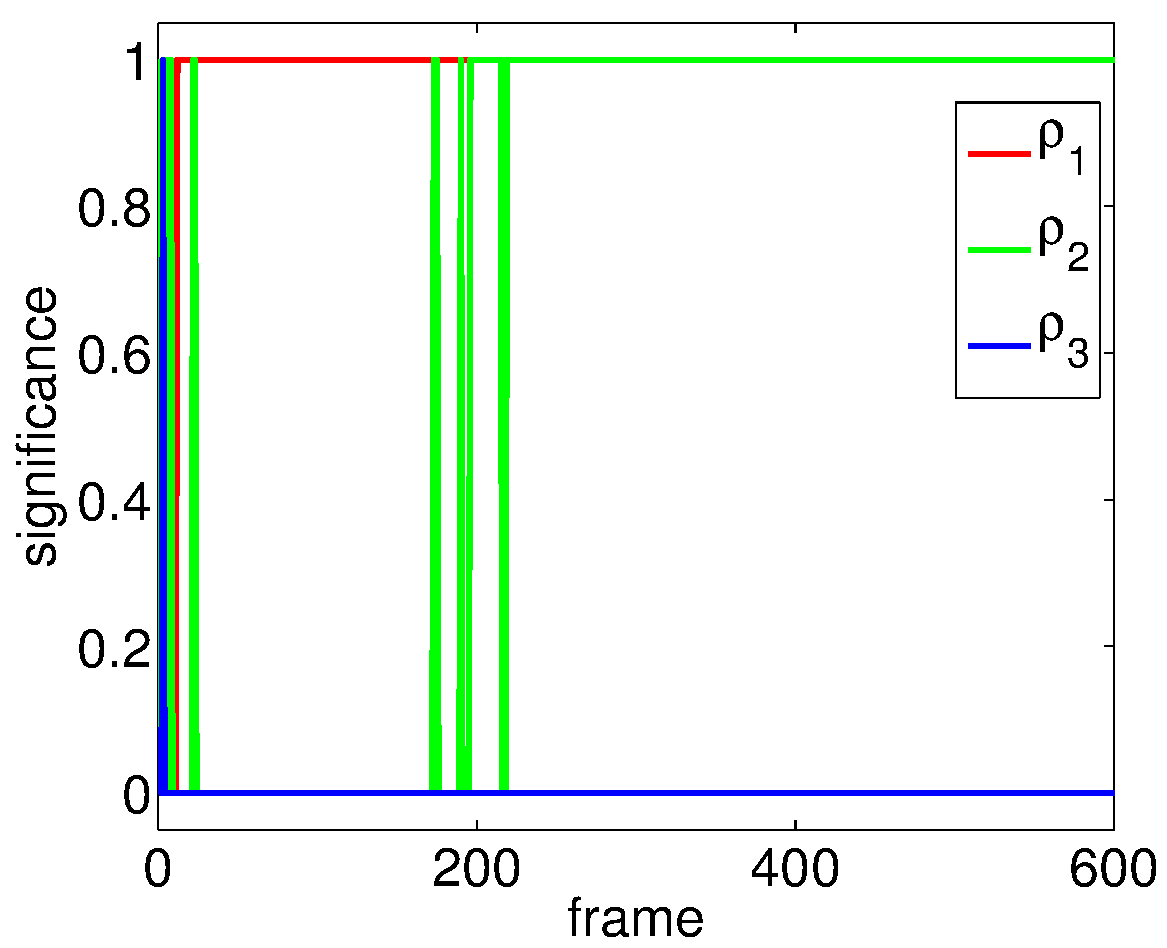
\includegraphics[width=0.45\textwidth]{figures/icca_sigs_miss.pdf}\\[2ex]
  \end{center}

\end{frame}

%%%%%%%%%%%%%%%%%%%%%%%%%%%%%%%%%%%%%%%%%%%%%%%%%%%%%%%%%%%%%%%%%%%%%%%%%%%%%%
\begin{frame}{Non-Gaussian Data}

\begin{Corr}[Non-Gaussian Data]
  Let $\mu_{Z_x}$ and $\mu_{Z_y}$ be the
  non-random compactly supported probability measures modeling the singular values of the
  noise matrices $X$ and $Y$. Let $b_x$ and $b_y$ be the supremums of the supports,
  respectively. Let $p,q,n\to\infty$ with $p/n\to c_x$ and $q/n\to c_y$. ICCA returns a
  consistent estimate of the number of correlated components under the following conditions
  \be
  \khaticca \convas k \text{ if } \min_{i=1,\dots,\kx}\tx_i>\frac{1}{D_{\mu_{Z_x}}(b_x^+)}
  \text{ and } \min_{i=1,\dots,\ky}\ty_i > \frac{1}{D_{\mu_{Z_y}}(b_y^+)}
  \ee
  where $D_{\mu_x}$ and $D_{\mu_y}$, the D-transforms of $\mu_{Z_x}$ and $\mu_{Z_y}$, are the
  functions, depending on $c_x$ and $c_y$.
\end{Corr}

\end{frame}



%%%%%%%%%%%%%%%%%%%%%%%%%%%%%%%%%%%%%%%%%%%%%%%%%%%%%%%%%%%%%%%%%%%%%%%%%%%%%%
\begin{frame}{Correlation Analysis Wish List}
  \addtocounter{framenumber}{-1}

  \begin{center}
    \textbf{Correlation Algorithm Wish List}\\[1ex]
\fcolorbox{black}[HTML]{F1F1F1}{\parbox{0.8\textwidth}{%
    \begin{enumerate}
    \item \textbf{Works in the sample deficient regime}
      \begin{itemize}
      \item {\textcolor{texthigh}{meaningful correlations \checkmark}}
      \item meaningful canonical vectors
      \end{itemize}
    \item {\textcolor{texthigh}{\textbf{Statistical test for correlations} \checkmark}}
      \begin{itemize}
      \item {\textcolor{texthigh}{consistency results \checkmark}}
      \end{itemize}
    \item {\textcolor{texthigh}{\textbf{Robustness} \checkmark}}
      \begin{itemize}
      \item {\textcolor{texthigh}{non-gaussian data \checkmark}}
      \item {\textcolor{texthigh}{missing data \checkmark}}
      \end{itemize}
    \item \textbf{Extension to more than 2 datasets}
    \item \textbf{Unification of performance analysis}
    \end{enumerate}
}}
\end{center}

\end{frame}


%%%%%%%%%%%%%%%%%%%%%%%%%%%%%%%%%%%%%%%%%%%%%%%%%%%%%%%%%%%%%%%%%%%%%%%
\begin{frame}{MCCA - Multiset CCA}

  \begin{center}
    \fcolorbox{black}[HTML]{F1F1F1}{\parbox{0.7\textwidth}{%
        \centering What if we have $m$ datasets $Y_1,\dots,Y_m$?  }}
  \end{center}

\vspace{1ex}

\textbf{Notation}
\begin{itemize}
\item covariance matrices: $R_{ij} = \E{y_iy_j^H}$
\item canonical vectors: $x_1,\dots,x_m$
\item canonical variates: $w_1,\dots, w_m$, $w_i=x_i^Hy_i$
\end{itemize}

\vspace{2ex}

\begin{equation*}
\Phi(x)=E[ww^H]=\left[\begin{array}{ccc} x_1^HR_{11}x_1 & \dots & x_1^HR_{1m}x_m \\ \vdots
    & \ddots & \vdots \\ x_m^HR_{m1}x_1 & \dots & x_m^HR_{mm}x_m\\ \end{array}\right]
\end{equation*}

\vspace{1ex}

\begin{center}
  \textbf{Optimization Problem}\\

  \fcolorbox{black}[HTML]{F1F1F1}{\parbox{0.5\textwidth}{%
      \be\ba
      &\underset{x}{\mathop{\rm optimize}} && J(\Phi(x))\\
      &\mathop{\rm subject to} && h(x,R)\\
      \ea\ee
    }}
\end{center}


\end{frame}

%%%%%%%%%%%%%%%%%%%%%%%%%%%%%%%%%%%%%%%%%%%%%%%%%%%%%%%%
\begin{frame}{MCCA - Multiset CCA}

  \begin{columns}[t]
    \begin{column}{0.5\textwidth}
      \centering\underline{\textbf{Ambiguity in Objective Function}}
      \begin{equation*}
        \begin{aligned}
          &\text{SUMCORR} &&\argmax_{x_1,\dots,x_m}\sum_{i=1}^m\sum_{j=1}^mx_i^HR_{ij}x_j\\[1ex]
          &\text{SSQCORR} &&\argmax_{x_1,\dots,x_m}\sum_{i=1}^m\sum_{j=1}^m\left(x_i^HR_{ij}x_j\right)^2\\[1ex]
          &\textcolor{texthigh}{\text{MAXVAR}} &&\textcolor{texthigh}{\argmax_{x_1,\dots,x_m}\lambda_1\left(\Phi(x)\right)}\\[1ex]
          &\textcolor{textred}{\text{MINVAR}} &&\textcolor{textred}{\argmin_{x_1,\dots,x_m}\lambda_m\left(\Phi(x)\right)}\\[1ex]
          &\text{GENVAR} &&\argmin_{x_1,\dots,x_m}\prod_{i=1}^m\lambda_i\left(\Phi(x)\right)\\[1ex]
        \end{aligned}
      \end{equation*}

    \end{column}
    \begin{column}{0.5\textwidth}
      \centering\underline{\textbf{Ambiguity in Constraint Function}}
      \begin{equation*}
        \begin{aligned}
          &\text{NORM} && \|x_i\|_2^2 =1\\[1ex]
          &\text{AVGNORM} &&\sum_{i=1}^m\|x_i\|_2^2 = m\\[1ex]
          &\textcolor{texthigh}{\text{VAR}} &&\textcolor{texthigh}{x_i^HR_{ii}x_i = 1}\\[1ex]
          &\text{AVGVAR} &&\sum_{i=1}^mx_i^HR_{ii}x_i = m\\[1ex]
        \end{aligned}
      \end{equation*}

    \end{column}
  \end{columns}

\end{frame}

%%%%%%%%%%%%%%%%%%%%%%%%%%%%%%%%%%%%%%%%%%%%%
\begin{frame}{MCCA - MAXVAR, VAR}

  \begin{center}
    \textbf{Objective Function}\\
    \fcolorbox{black}[HTML]{F1F1F1}{\parbox{0.4\textwidth}{%
        \be\ba
        &\argmax_{x_1,\dots,x_m}&&\lambda_1\left(\Phi(x)\right)\\
        &\text{subject to} &&x_i^HR_{ii}x_i = 1, \forall i
        \ea\ee
      }}
    \end{center}

  \begin{itemize}
  \item Let $V_i$ be the right singular vectors of dataset $Y_i$
  \end{itemize}

  \be
  \Cmcca=\left[\begin{array}{cccc} I_{d_1} & V_1^HV_2 & \cdots & V_1^HV_m\\
      V_2^HV_1 & I_{d_2} & \cdots & V_2^HV_m\\
      \vdots & \vdots & \ddots & \vdots\\
      V_m^HV_1 & V_m^HV_2 & \cdots & I_{d_m}\end{array}\right]
  \ee


  \begin{itemize}
  \item Let $\Cmcca = FKF^H$ be eigenvalue decomposition
  \item $\rho^{(j)} = k_j$
  \item $x_i = R_{ii}^{-1/2}f_i$
  \end{itemize}

\end{frame}

\begin{frame}{MAXVAR for CCA}

\textbf{Two dataset setting}
\be\ba
&C_{\text{cca}} && = \left[\begin{array}{c}V_1^H\\V_2^H\end{array}\right]\left[\begin{array}{cc}V_1 &
    V_2\end{array}\right] \\
&&&= \left[\begin{array}{cc}I_{d_1} &
    V_1^HV_2\\ V_2^HV_1 & I_{d_2}\end{array}\right]\\
&&&= \left[\begin{array}{cc}F & -F\\ G & G\end{array}\right]
\left[\begin{array}{cc}I + \left(KK^H\right)^{-1/2} & 0\\ 0 & I - \left(K^HK\right)^{-1/2}\end{array}\right]
\left[\begin{array}{cc}F & -F\\ G & G\end{array}\right]^H
\ea\ee

\vspace{2ex}

\textbf{Insights}
\begin{itemize}
\item Eigenvalues come in pairs $\left\{1+k_i,1-k_i,\right\}$
\item Perfect correlation implies $\lambda_{\text{max}}=2$, $\lambda_{\text{min}} = 0$
\item Eigenvectors have specific structure
\item MINVAR solves the same problem!
\item Correlation implies \textit{ALL} datasets correlated!
\end{itemize}


\end{frame}

%%%%%%%%%%%%%%%%%%%%%%%%%%%%%%%%%%%%%%%%%%%%%
\begin{frame}{MCCA - Ambiguity Example}

\textbf{3 Dataset Example}
\be
\Cmcca^{(1)} =  \left[\begin{array}{ccc}1 &  1 & 0\\ 1 & 1&0\\  0 & 0 &
    1 \end{array}\right],\,\,\,\, \Cmcca^{(2)} =  \left[\begin{array}{ccc}1 &  0.5 & 0.5\\ 0.5 &
    1&0.5\\  0.5 & 0.5 & 1 \end{array}\right]
\ee

\begin{itemize}
\item Both have $\lambda_1=2$
\item $u^{(1)} = \frac{1}{\sqrt{2}}\left[1, 1, 0\right]^T$
\item $u^{(2)}=\frac{1}{\sqrt{3}}\left[1,1,1\right]^T$
\end{itemize}

\vspace{3ex}

\textbf{Insights}
\begin{itemize}
\item Eigenvalue detects correlation
\item Eigenvector reveals structure
\end{itemize}

      \begin{center}
        \textbf{Proposed correlation statistic}\\
        \fcolorbox{black}[HTML]{F1F1F1}{\parbox{0.4\textwidth}{%
            \be
            \widehat{\rho}^{(i)} = \lambda_i\left(\Cmcca - I\right)
            \ee
          }}
      \end{center}


\end{frame}

\begin{frame}{Informative MCCA}

  \textbf{Idea - Trim right singular vectors}
  \begin{itemize}
  \item  $\Ucir_j = \widehat{U}_j\left(:,1:\widehat{k}_j\right)$
  \item  $\Vcir_j = \widehat{V}_j\left(:,1:\widehat{k}_j\right)$
  \item $\Ucir = \blkdiag(\Ucir_1,\dots,\Ucir_m)$
  \item  $\Vcir =\left[\Vcir_1,\dots \Vcir_m\right]$
  \end{itemize}

\begin{center}
  \fcolorbox{black}[HTML]{F1F1F1}{\parbox{0.4\textwidth}{%
      \be
      \Cmccatil = \Ucir\Vcir^H\Vcir\Ucir^H.
      \ee
}}
\end{center}

\vspace{2ex}

\begin{center}
\textbf{Estimate the number of correlations}\\[1ex]
  \fcolorbox{black}[HTML]{F1F1F1}{\parbox{0.4\textwidth}{%
      \be
      \widehat{t}_{\text{imcca}} = \sum_{i=1}^{\widehat{k}}
      \indicator_{\left\{\widehat{\kappa}_i > \tau_{\text{imcca}}^\alpha\right\}}, 
      \ee
    }}
\end{center}

\end{frame}

%%%%%%%%%%%%%%%%%%%%%%%%%%%%%%%%%%%%%%%%%%%%%
\begin{frame}{\href{run:/home/user/Documents/thesis_vids/mcca_flashing.mp4}{MCCA and
      IMCCA Demonstration}} 



    \begin{center}
      \textbf{MCCA Correlations}\hspace{20ex}\textbf{IMCCA Correlations}
        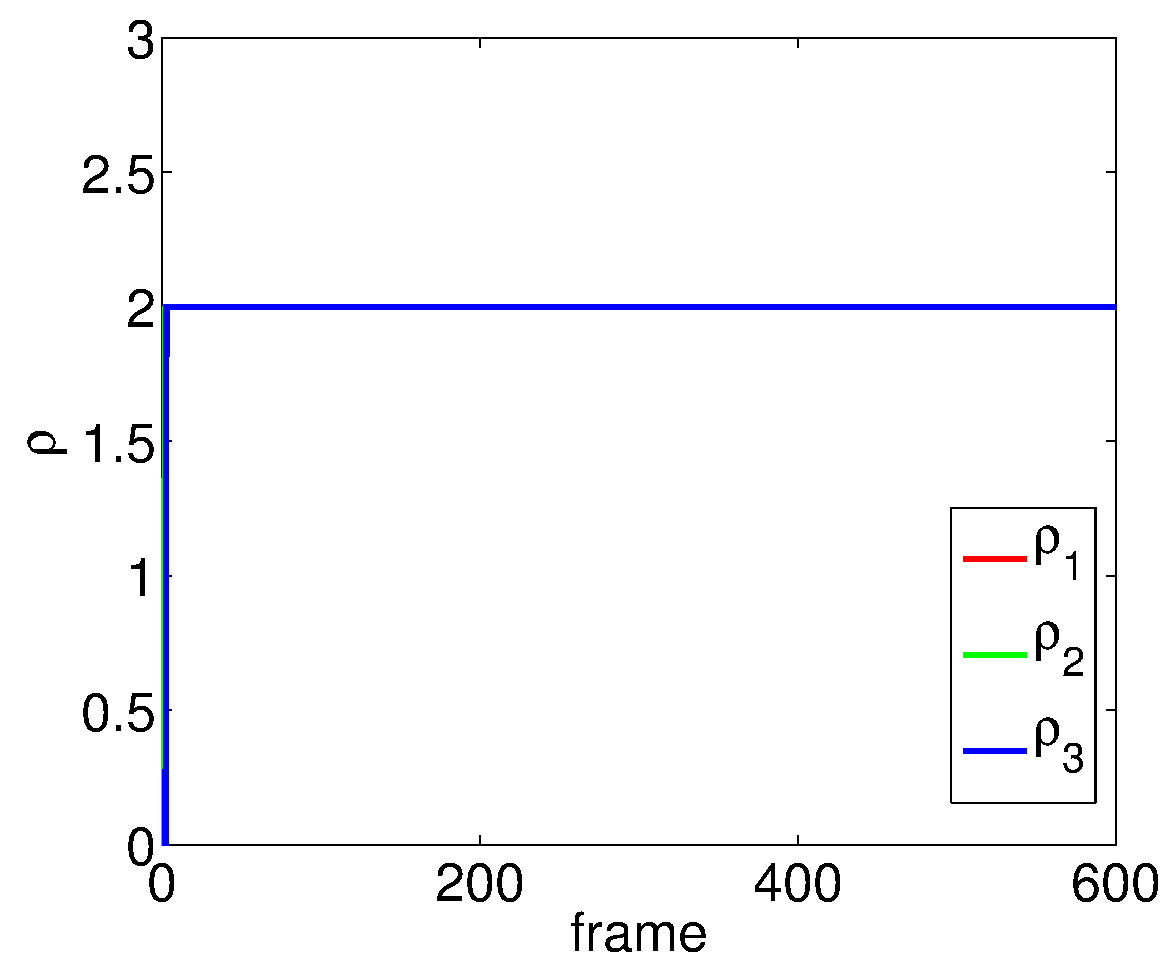
\includegraphics[width=0.45\textwidth]{figures/mcca_cca_corrs.pdf}\hspace{2ex}
        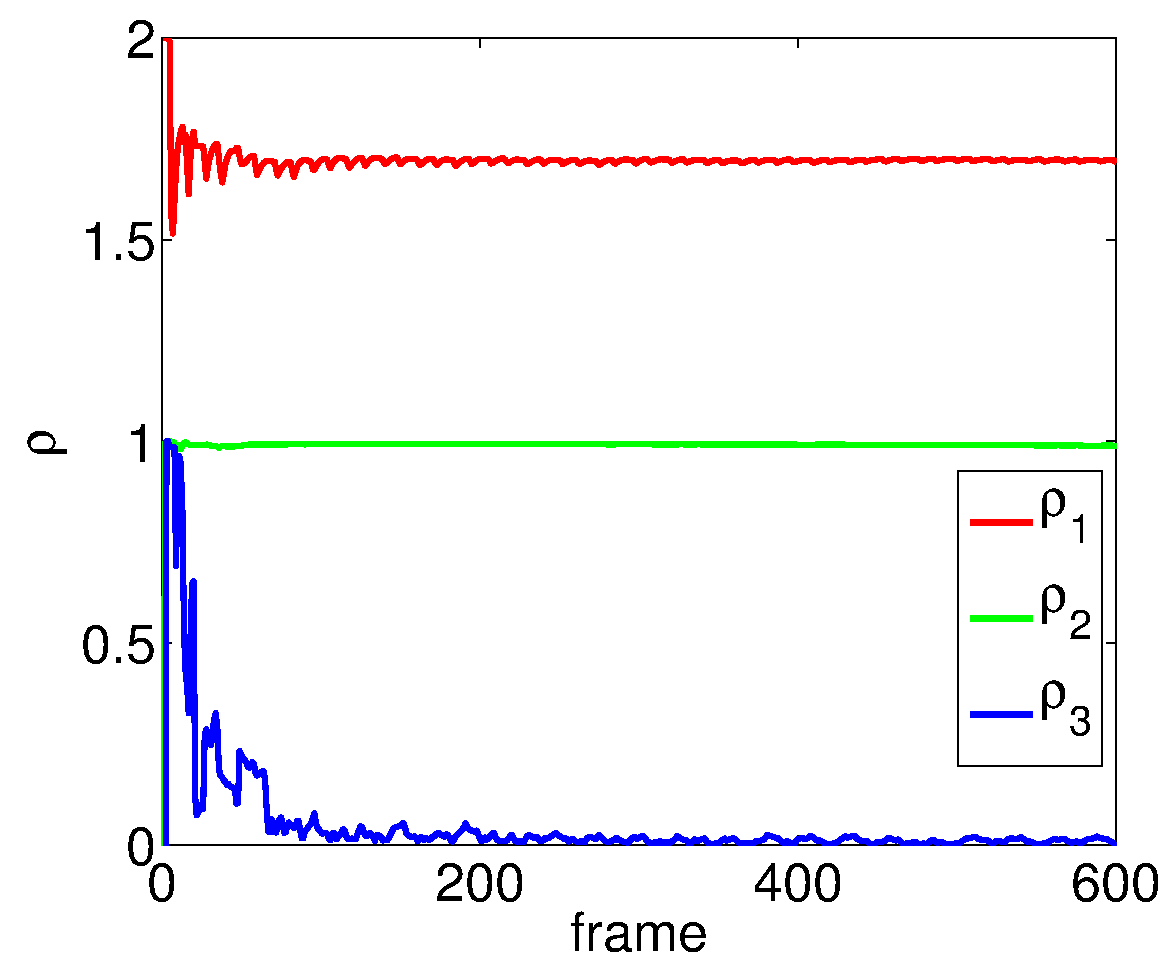
\includegraphics[width=0.45\textwidth]{figures/mcca_icca_corrs.pdf}
    \end{center}

\end{frame}

%%%%%%%%%%%%%%%%%%%%%%%%%%%%%%%%%%%%%%%%%%%%%%%%%%%%%%%%%%%%%%%%%%%%%%%%%%%%%%
\begin{frame}{Correlation Analysis Wish List}
  \addtocounter{framenumber}{-1}

  \begin{center}
    \textbf{Correlation Algorithm Wish List}\\[1ex]
\fcolorbox{black}[HTML]{F1F1F1}{\parbox{0.8\textwidth}{%
    \begin{enumerate}
    \item \textbf{Works in the sample deficient regime}
      \begin{itemize}
      \item {\textcolor{texthigh}{meaningful correlations \checkmark}}
      \item meaningful canonical vectors
      \end{itemize}
    \item {\textcolor{texthigh}{\textbf{Statistical test for correlations} \checkmark}}
      \begin{itemize}
      \item {\textcolor{texthigh}{consistency results \checkmark}}
      \end{itemize}
    \item {\textcolor{texthigh}{\textbf{Robustness} \checkmark}}
      \begin{itemize}
      \item {\textcolor{texthigh}{non-gaussian data \checkmark}}
      \item {\textcolor{texthigh}{missing data \checkmark}}
      \end{itemize}
    \item \textcolor{texthigh}{\textbf{Extension to more than 2 datasets} \checkmark}
    \item \textbf{Unification of performance analysis}
    \end{enumerate}
}}
\end{center}

\end{frame}


%%%%%%%%%%%%%%%%%%%%%%%%%%%%%%%%%%%%%%%%%%%%%%%%%%%%%%%%%%%%%%%%%%%%%%%%%%%%%%
\begin{frame}{Canonical Vector Estimation}

\textbf{Data SVDs}
\begin{itemize}
\item $X=\Uxhat\Sigxhat\Vxhat^H$
\item $X=\Uxcir\Sigxcir\Vxcir^H$
\item $\Uktil$ left singular vectors of $\Kxytil$
\item $\widetilde{U}_{\widetilde{K}}$ left singular vectors of $\Cccahat$
\item $\Uktilhat$ left singular vectors of $\Ciccahat$
\end{itemize}

\vspace{3ex}

\begin{table}[t]
\centering
\begin{tabular}{l|l}\toprule
Estimate & \\
\midrule
\textbf{Population}  & $W_x = \Ux\left(\Tx + I_{\kx}\right)^{-1/2}\Uktil$\\[1ex]
\textbf{CCA} & $\widehat{W}_x^{\text{cca}} =
\Uxhat\left(\Sigxhat\right)^{-1}\widehat{U}_{\widetilde{K}}$\\[1ex]
\textbf{ICCA} & $\widehat{W}_x^{\text{icca}} = \Uxcir\Sigxcir^{-1}\Ukcir$\\[1ex]
\textbf{\iccap} &$\widehat{W}_x^{\text{icca+}} = \Uxcir\Lambda_x^{\text{opt}}\Ukcir$\\[1ex]
\bottomrule
\end{tabular}
\end{table}

\end{frame}


%%%%%%%%%%%%%%%%%%%%%%%%%%%%%%%%%%%%%%%%%%%%%%%%%%%%%%%%%%%%%%%%%%%%%%%%%%%%%% 
\begin{frame}{Canonical Vector Accuracy Experiment}
  \begin{center}
    \textbf{ICCA}\hspace{23ex}\textbf{\iccap}\phantom{blah}\\
    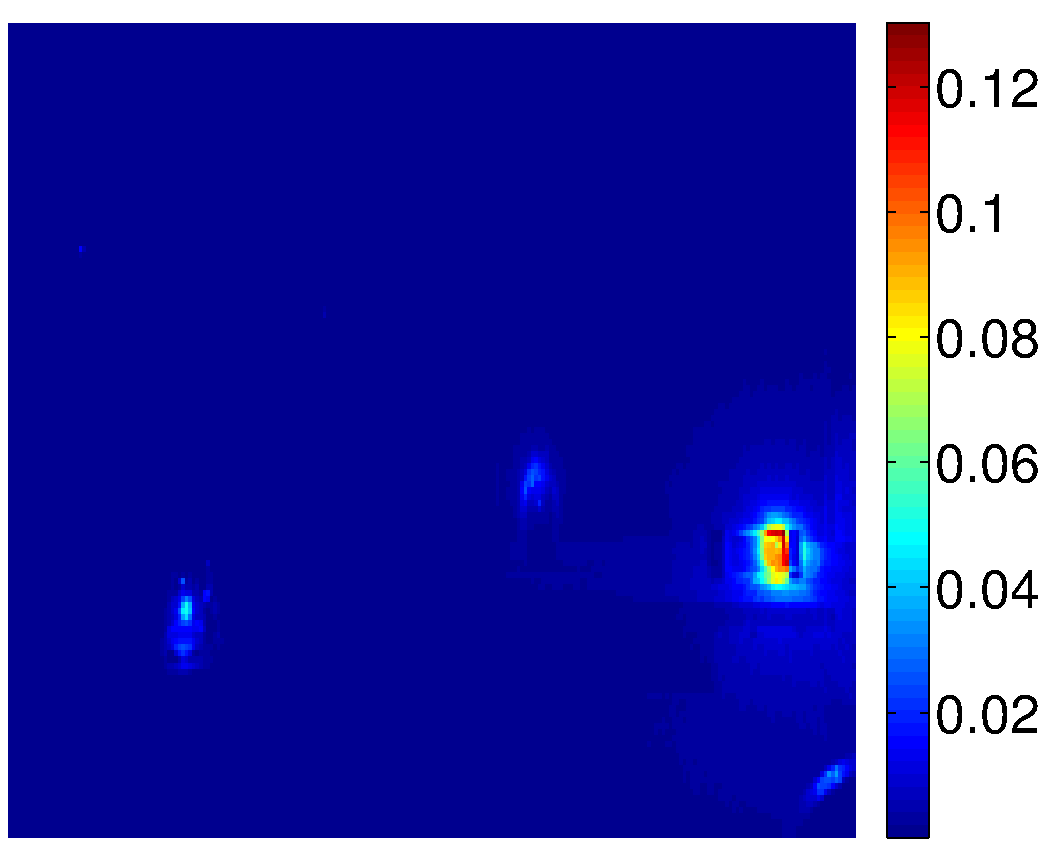
\includegraphics[width=0.35\textwidth]{figures/flashing1_left1_icca.pdf}\hspace{2ex}
    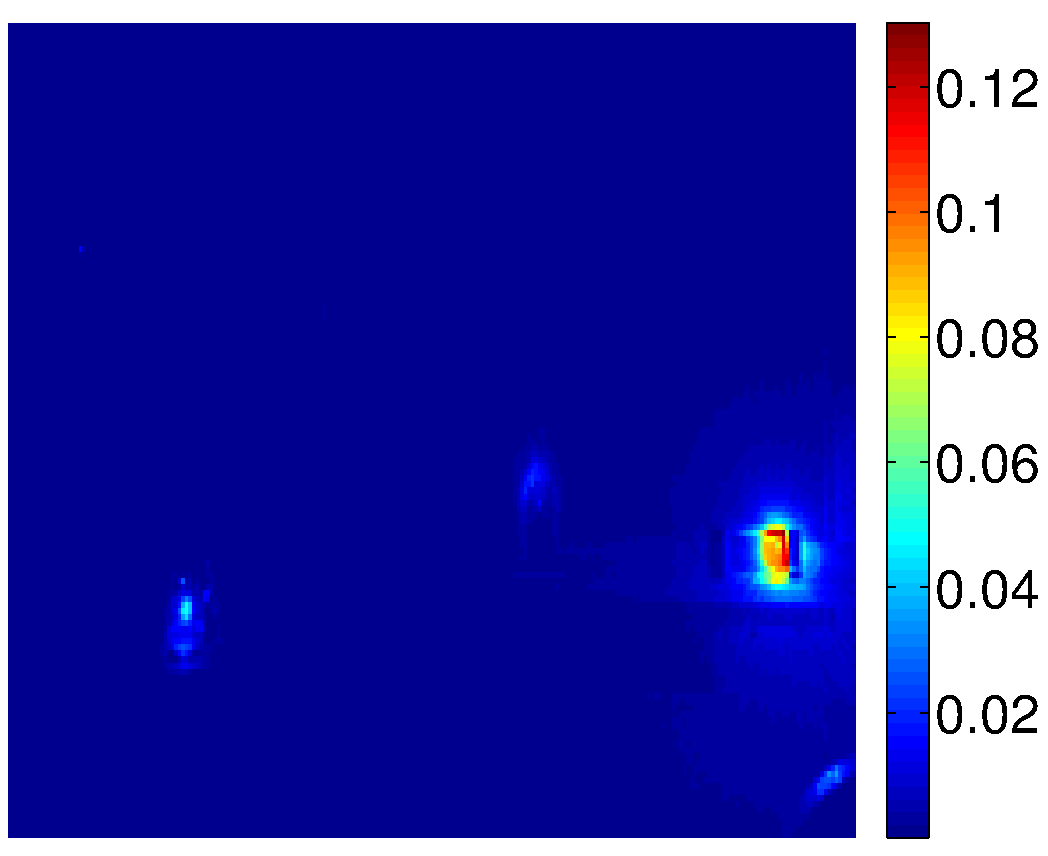
\includegraphics[width=0.35\textwidth]{figures/flashing1_left1_opt.pdf}\\[2ex]
    \textbf{CCA}\hspace{23ex}\textbf{ICCA - \iccap}\\
    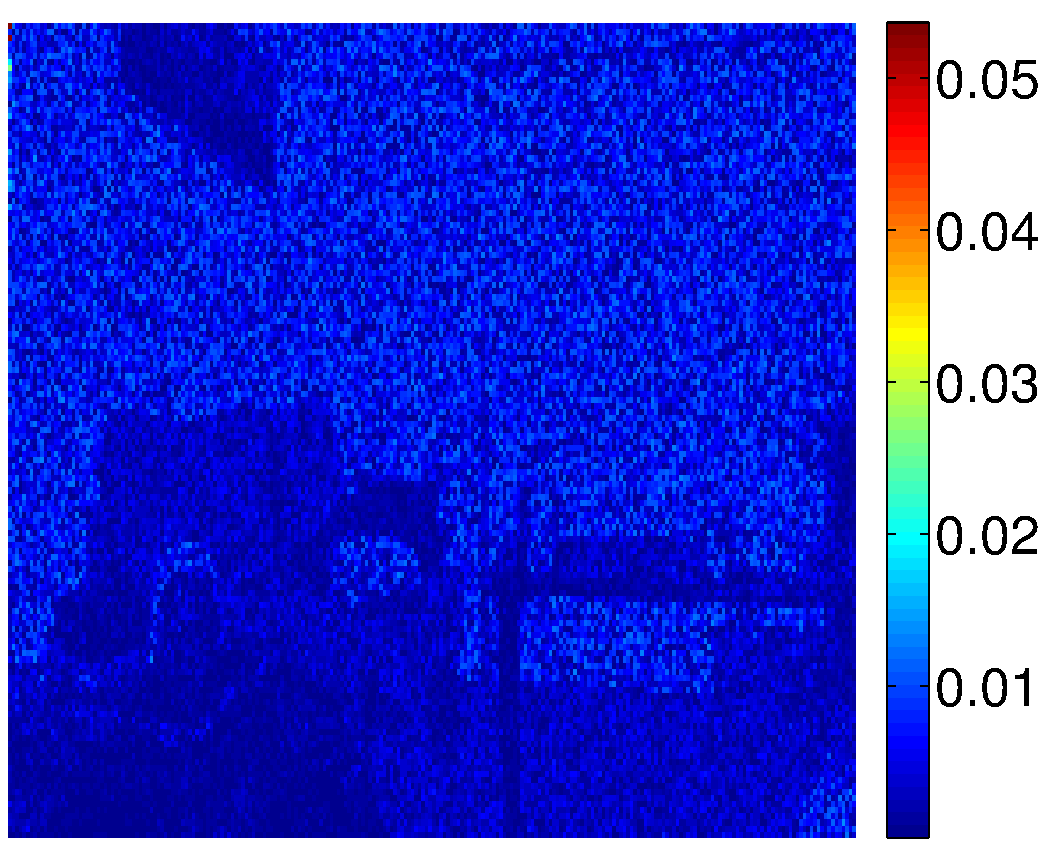
\includegraphics[width=0.35\textwidth]{figures/flashing1_left1_cca.pdf}\hspace{2ex}
    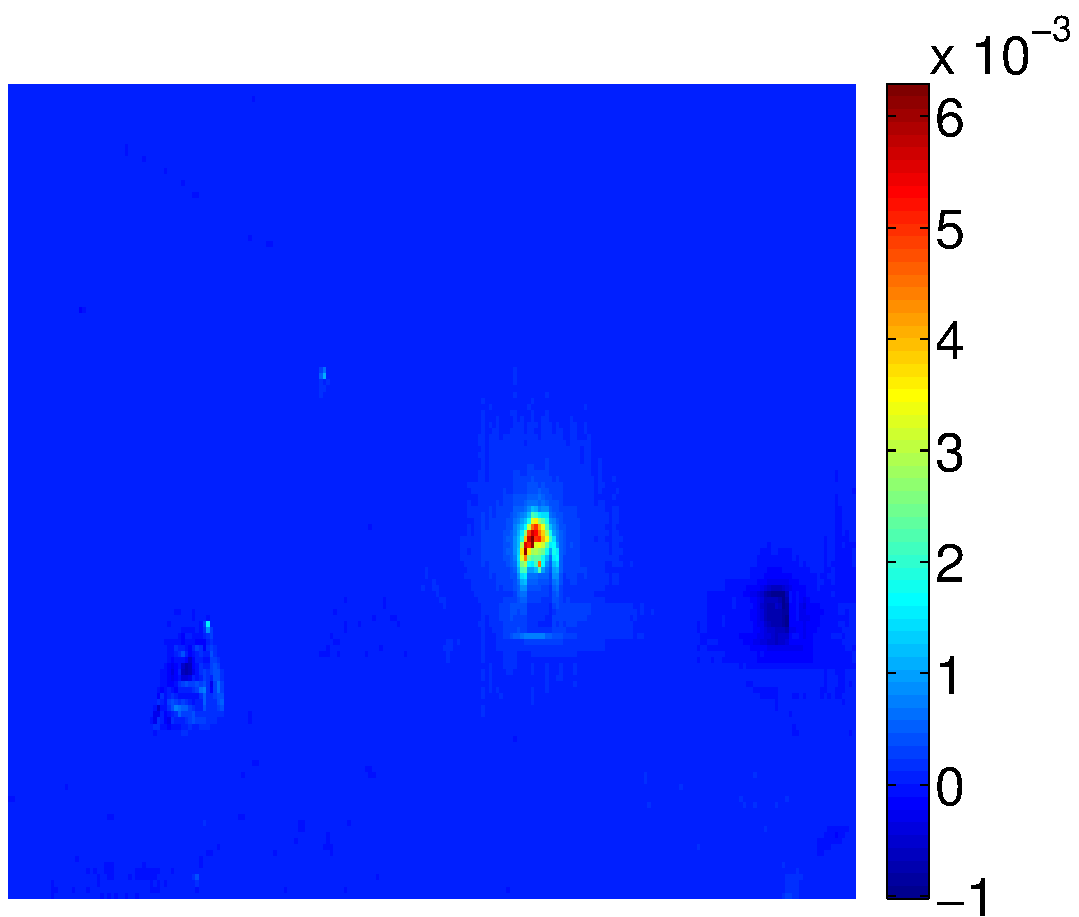
\includegraphics[width=0.35\textwidth]{figures/flashing1_left1_diff_icca.pdf}
  \end{center}
\end{frame}

%%%%%%%%%%%%%%%%%%%%%%%%%%%%%%%%%%%%%%%%%%%%%%%%%%%%%%%%%%%%%%%%%%%%%%%%%%%%%%
\begin{frame}{Correlation Analysis Wish List}
  \addtocounter{framenumber}{-1}

  \begin{center}
    \textbf{Correlation Algorithm Wish List}\\[1ex]
\fcolorbox{black}[HTML]{F1F1F1}{\parbox{0.8\textwidth}{%
    \begin{enumerate}
    \item \textcolor{texthigh}{\textbf{Works in the sample deficient regime} \checkmark}
      \begin{itemize}
      \item {\textcolor{texthigh}{meaningful correlations \checkmark}}
      \item \textcolor{texthigh}{meaningful canonical vectors \checkmark}
      \end{itemize}
    \item {\textcolor{texthigh}{\textbf{Statistical test for correlations} \checkmark}}
      \begin{itemize}
      \item {\textcolor{texthigh}{consistency results \checkmark}}
      \end{itemize}
    \item {\textcolor{texthigh}{\textbf{Robustness} \checkmark}}
      \begin{itemize}
      \item {\textcolor{texthigh}{non-gaussian data \checkmark}}
      \item {\textcolor{texthigh}{missing data \checkmark}}
      \end{itemize}
    \item \textcolor{texthigh}{\textbf{Extension to more than 2 datasets} \checkmark}
    \item \textbf{Unification of performance analysis}
    \end{enumerate}
}}
\end{center}

\end{frame}

%%%%%%%%%%%%%%%%%%%%%%%%%%%%%%%%%%%%%%%%%%%%%%%%%%%%%%%%%%%%%%%%%%%%%%%%%%%%%%
\begin{frame}{Analysis of $XY^H$ - Chpt. 6}

  \textbf{Recall key insight}
  \begin{itemize}
  \item $k = \Rank(\Ccca) = \Rank(\Rxy)$
  \end{itemize}

  \vspace{1ex}
  
  \begin{center}
    \textbf{Simulation of $\sigma_i(XY^H)$ with noise}\\
    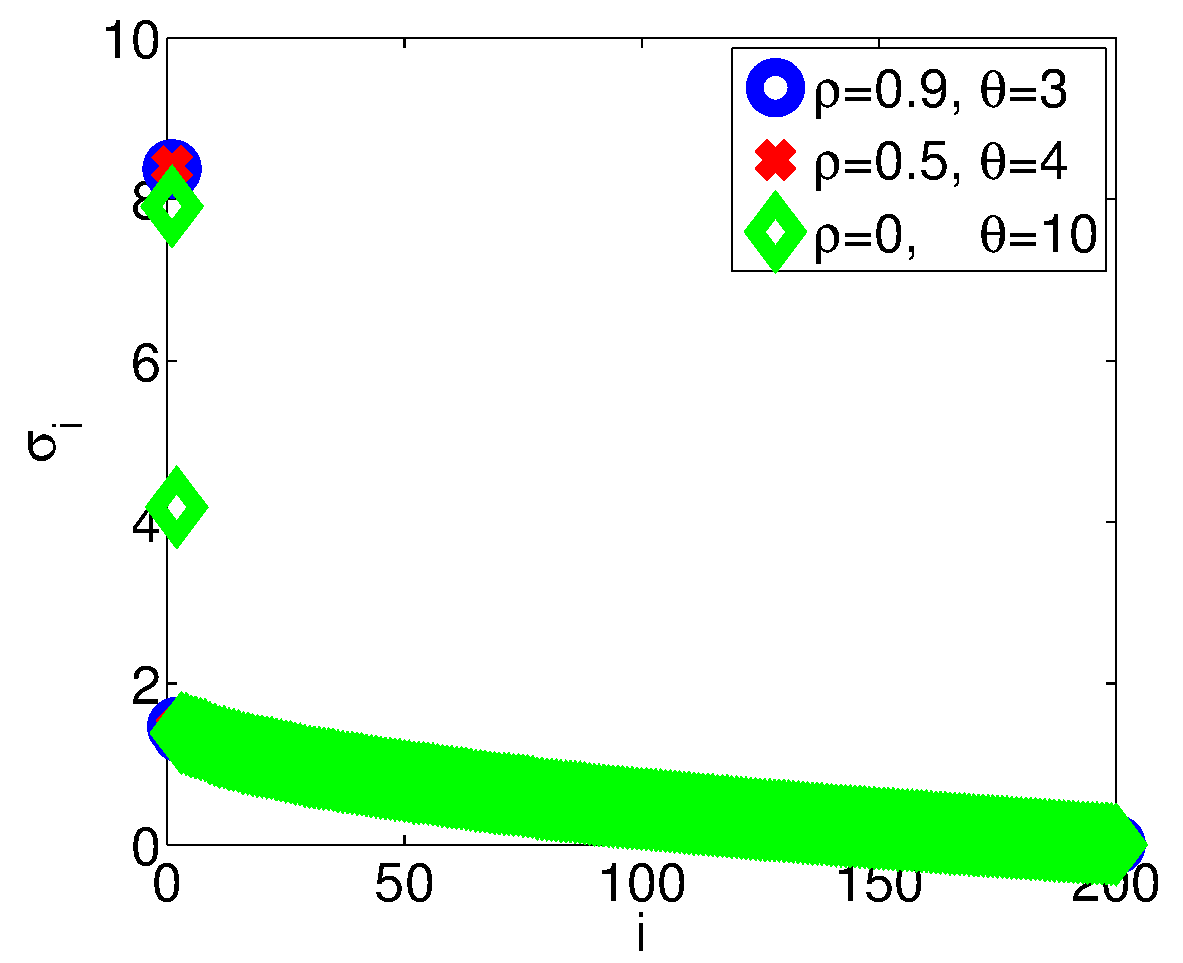
\includegraphics[width=0.45\textwidth]{figures/xy_motiv_pres.pdf}
  \end{center}

  \vspace{1ex}

  \textbf{Let's use SNR estimates}
  \begin{itemize}
  \item Pre-whiten the datasets 
  \item This is exactly CCA/ICCA!!
  \end{itemize}

\end{frame}

\begin{frame}{Analysis of $XY^H$ - Chpt. 6}

  \textbf{Contributions


\end{frame}


\end{document}
